\documentclass[12pt]{scrartcl}

 

\usepackage[utf8]{inputenc}

\usepackage[T1]{fontenc}

\usepackage{lmodern}

\usepackage[ngerman]{babel}

\usepackage{amsmath}

\usepackage{graphicx}

\usepackage{float}


 

\title{Versuch WP1\\ Polarisation von Licht}

\author{Frederik Strothmann, Henrik Jürgens}

\date{\today}


\begin{document}


 %deckblatt erstellen

\maketitle
\tableofcontents
\newpage

%einleitung zu dem experiment

\section{Einleitung}
Mit einer Photozelle untersuchen wir, wie sich Licht verhält, wenn es durch Polarisationsfilter tritt (Gesetz von Malus), an einem trüben Medium (Tröpfchen-Suspension in Wasser) gestreut wird oder an einer Glasplatte reflektiert wird (Brewsterscher Winkel).
Danach werden die Eigenschaften von zirkular oder elliptisch polarisierten Lichtwellen untersucht sowie ihre Wechselwirkung mit Materie (Cellophan, Zuckerlösung zur Demonstration der optischen Aktivität, Metallspiegel). 

%versuchsaufbau mit skizze

\section{Versuchsaufbau}
Der Versuchsaufbau besteht aus einer optischen Bank, einem Intensitätsmessgerät und einer Photozelle, welche zur Bestimmung der Intensität verwendet werden. Uns stehen für die Versuche eine Glühlampe, Polarisatoren, eine Blende, ein PVP, ein $\frac{\lambda}{4}$-Plättchen, eine Küvette und ein Plexiglasblock zu Verfügung. Für die Befestigung an der optischen Bank verwenden wir anschraubbare höhenverstellbare Halterungen, einen kleinen Tisch für die Küvette und einen kleinen Tisch mit Winkelmesser für den Plexiglasblock.

\begin{figure}[H]
\centering
    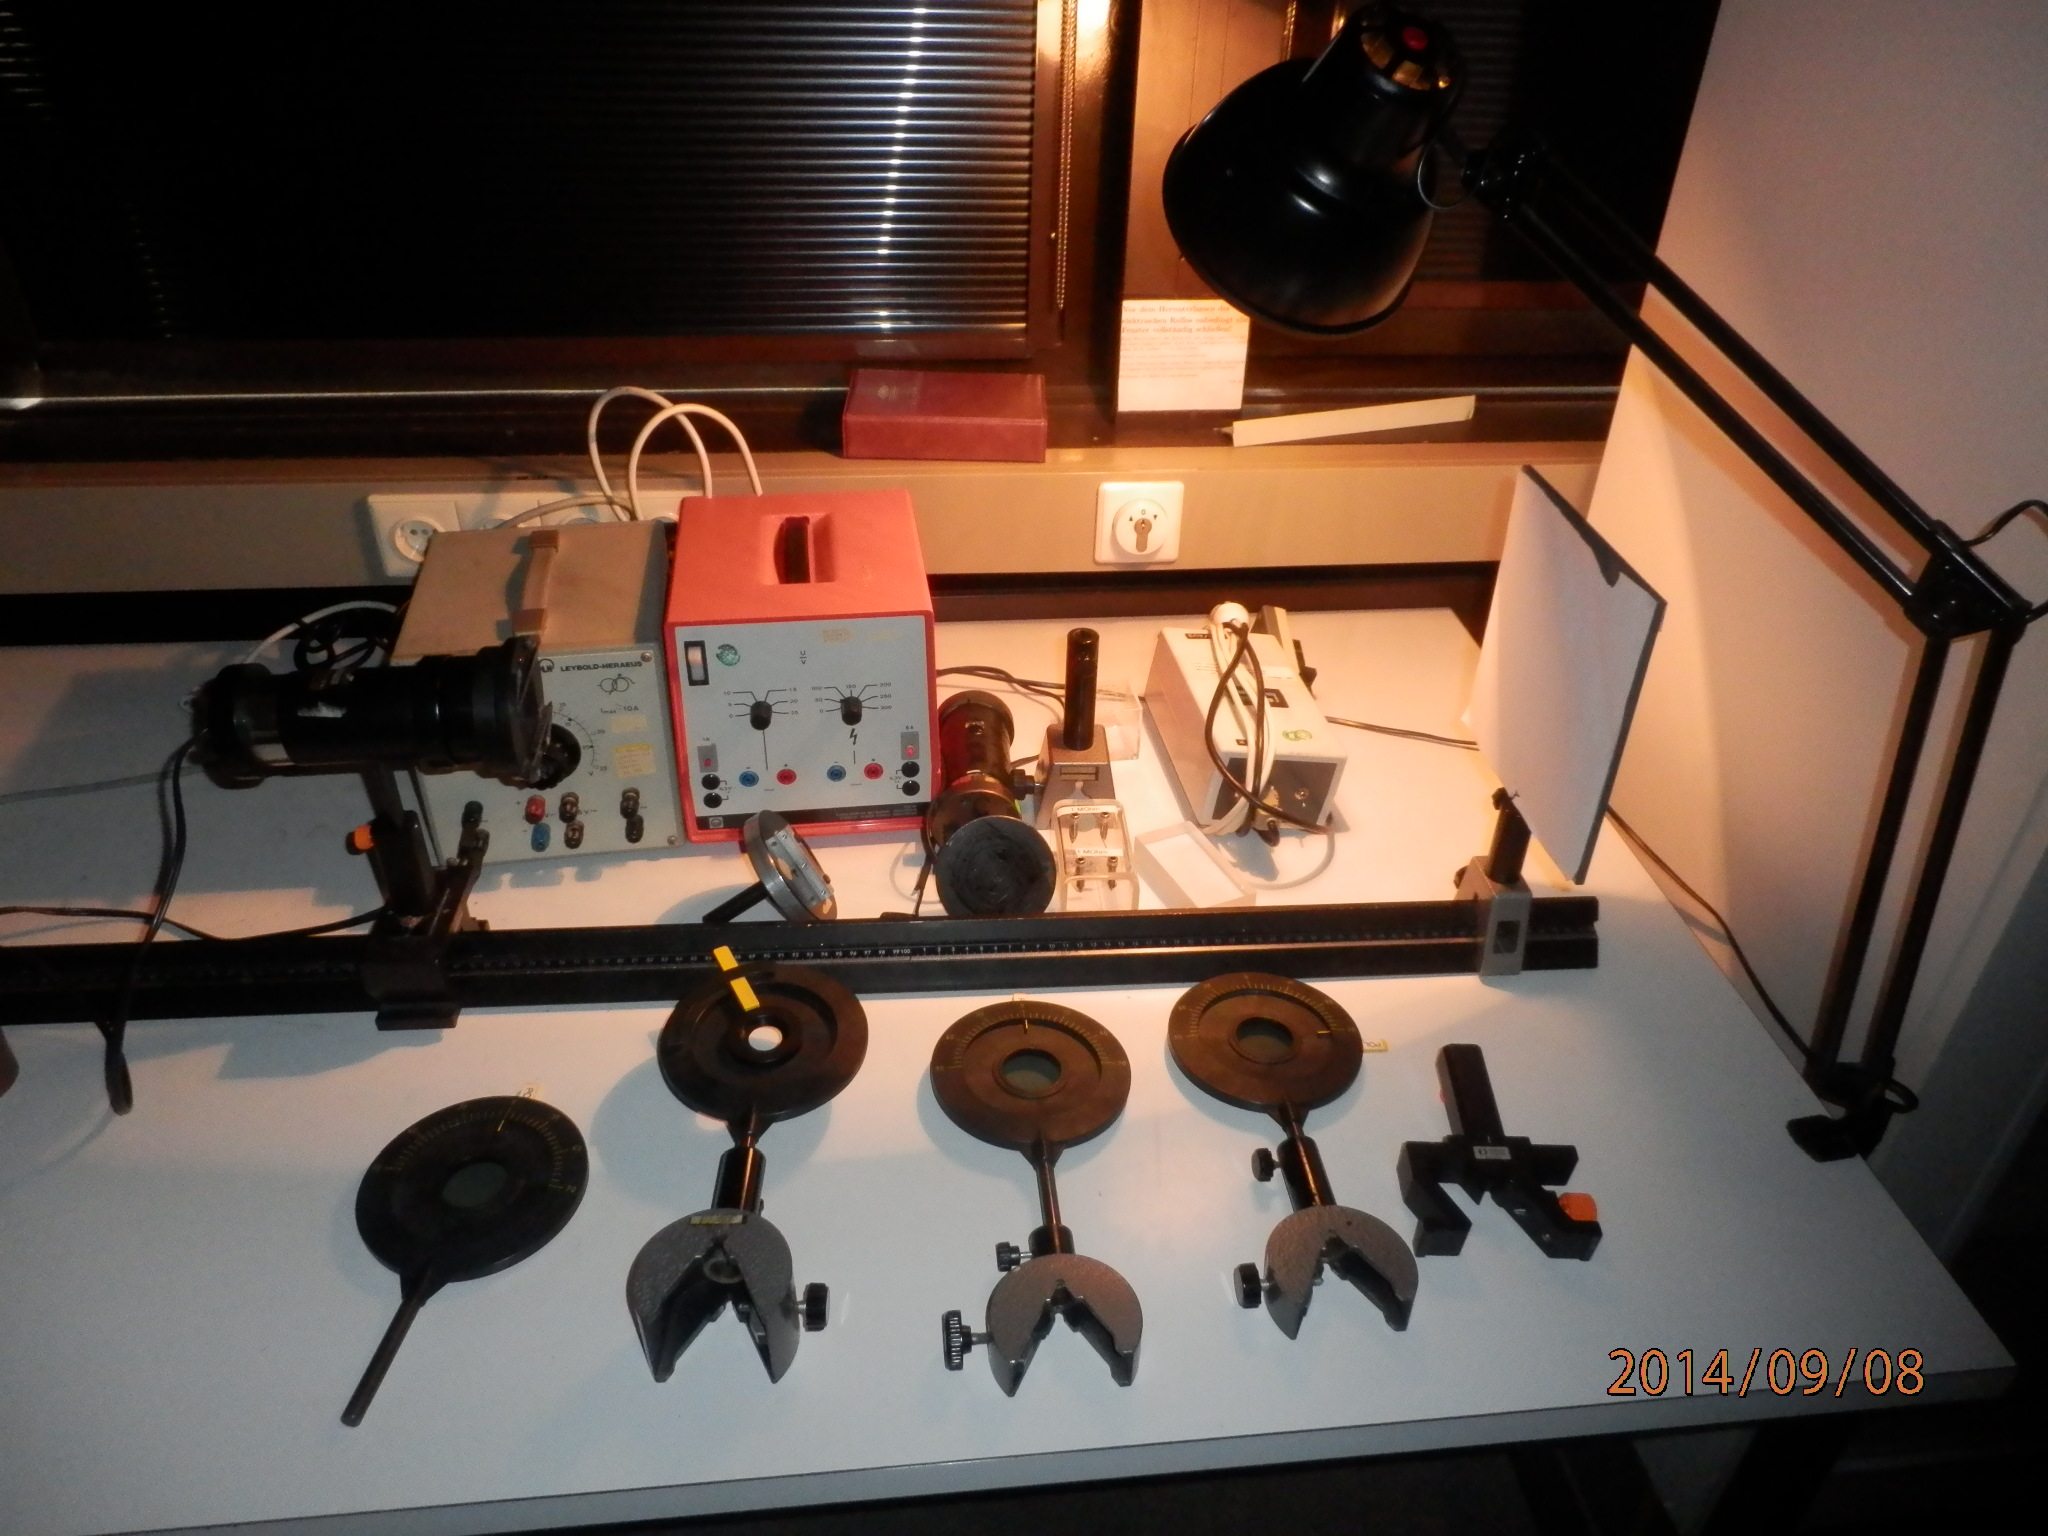
\includegraphics[scale = 0.1]{aufbau.JPG}
  	\caption[Foto des Versuchsaufbaus]{Foto des Versuchsaufbaus}
  \label{fig:a_1}
\end{figure}




\section{Versuch WO1.1: Verifizierung des Malusschen Gesetzes}
\subsection{Versuchsdurchführung}

\begin{figure}[H]
\centering
    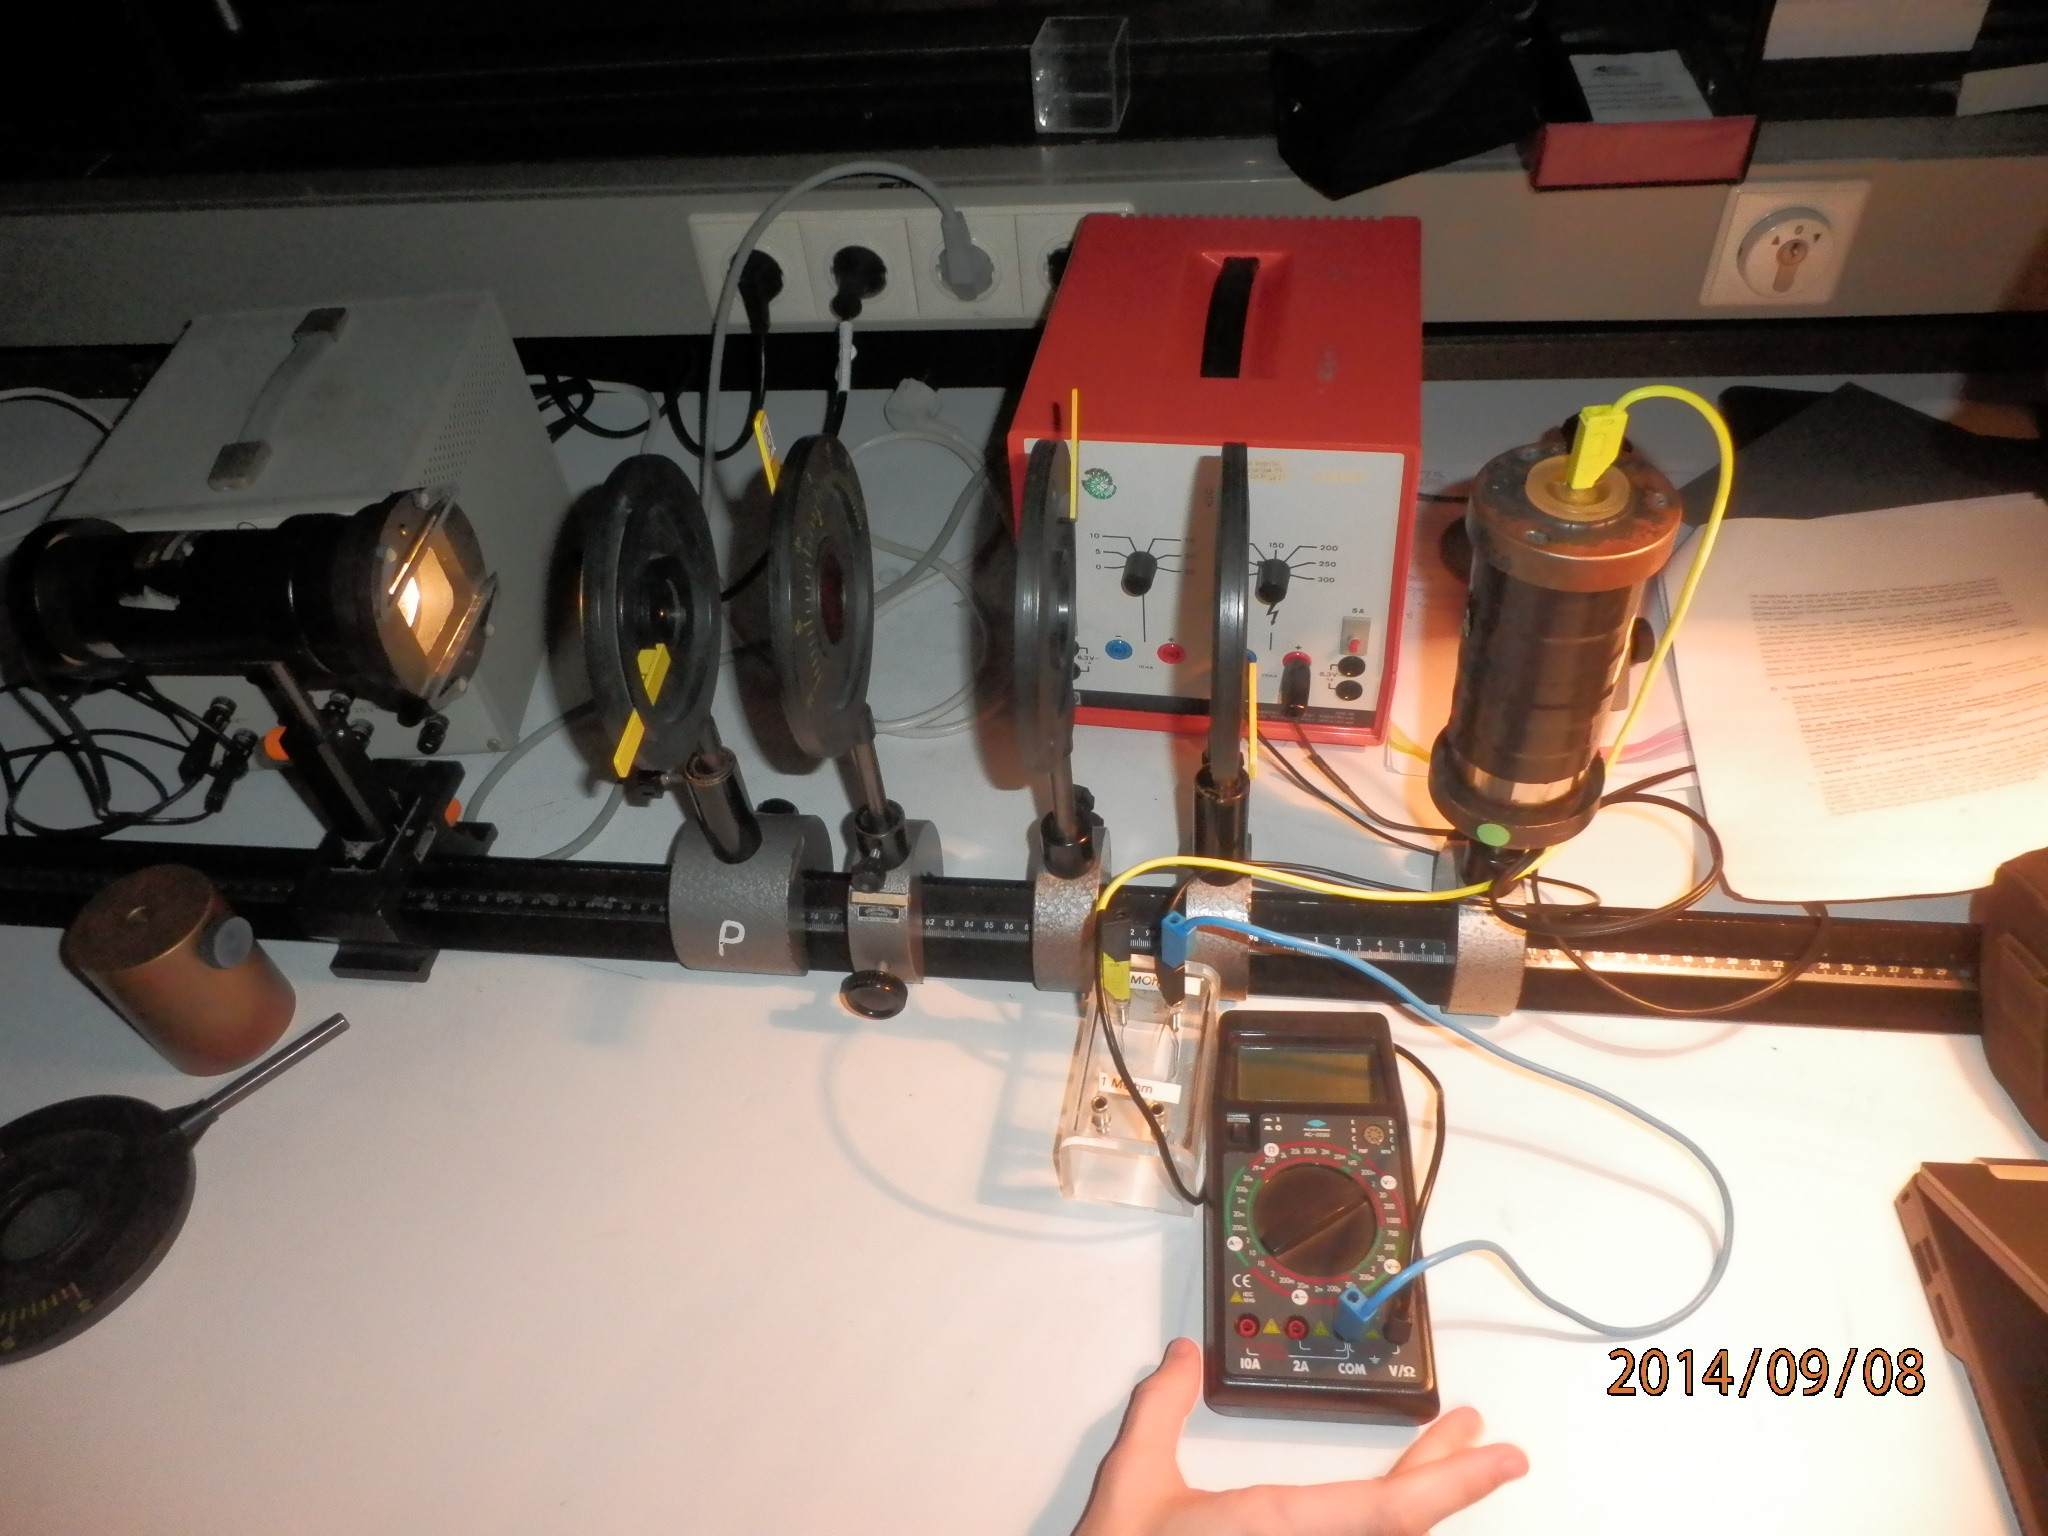
\includegraphics[scale = 0.1]{aufgabe_1.JPG}
  	\caption[Foto des Versuchsaufbaus für die erste Aufgabe]{Foto des Versuchsaufbaus für die erste Aufgabe}
  \label{fig:aufgabe_1}
\end{figure}

\subsubsection{Praktische Durchführung}
Wir bauen auf einer optischen Bank die in 
der folgenden Abbildung skizzierte Anordnung auf.
%Bitte Abbildung 4 aus der Versuchsbeschreibung einfügen

\begin{figure}[H] 
  \centering
    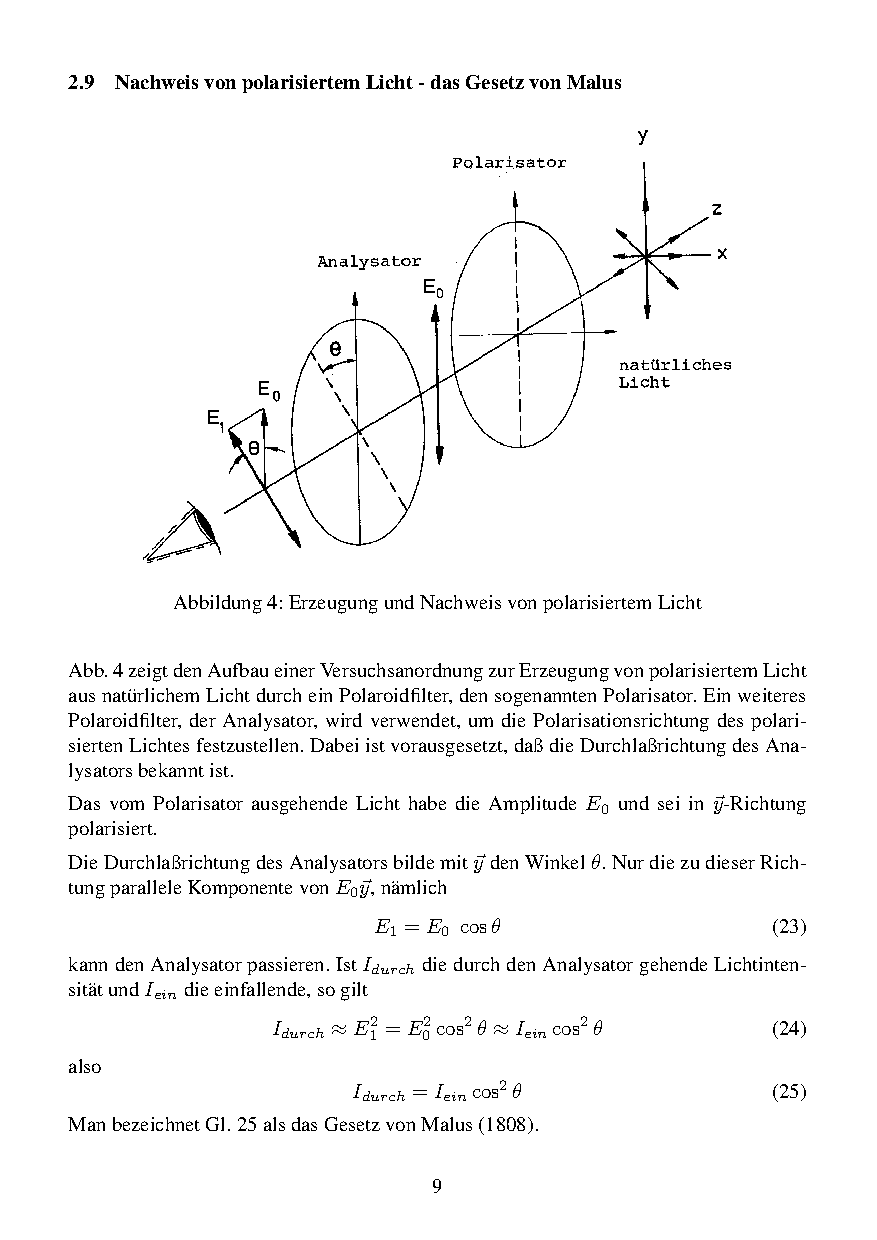
\includegraphics[trim = 0mm 110mm 0mm 20mm, clip, scale = 1]{abb_4.pdf}
  	\caption[Skizze des Aufbaus, auf der optische Bank]{Skizze des Aufbaus, auf der optische Bank\footnotemark}
  \label{fig:abb_4}
\end{figure}
\footnotetext{Abbildung entnommen von http://www.atlas.uni-wuppertal.de/~kind/wp1.pdf Seite 9 am 07.09.2014}

Wir verwenden eine Glühlampe mit Kondensor, der so eingestellt ist, daß das von der Glühlampe ausgehende Licht auf die Photozelle fokussiert ist. Eine Irisblende zwischen Kondensor und Polarisator dient der Regelung der Lichtintensität. Die
Lichintensität wird so eingestellt, dass der Photostrom $I_A$ der Photozelle 
%(siehe Abb. 3 und Gleichungen 21, 22)

\begin{figure}[H] 
  \centering
    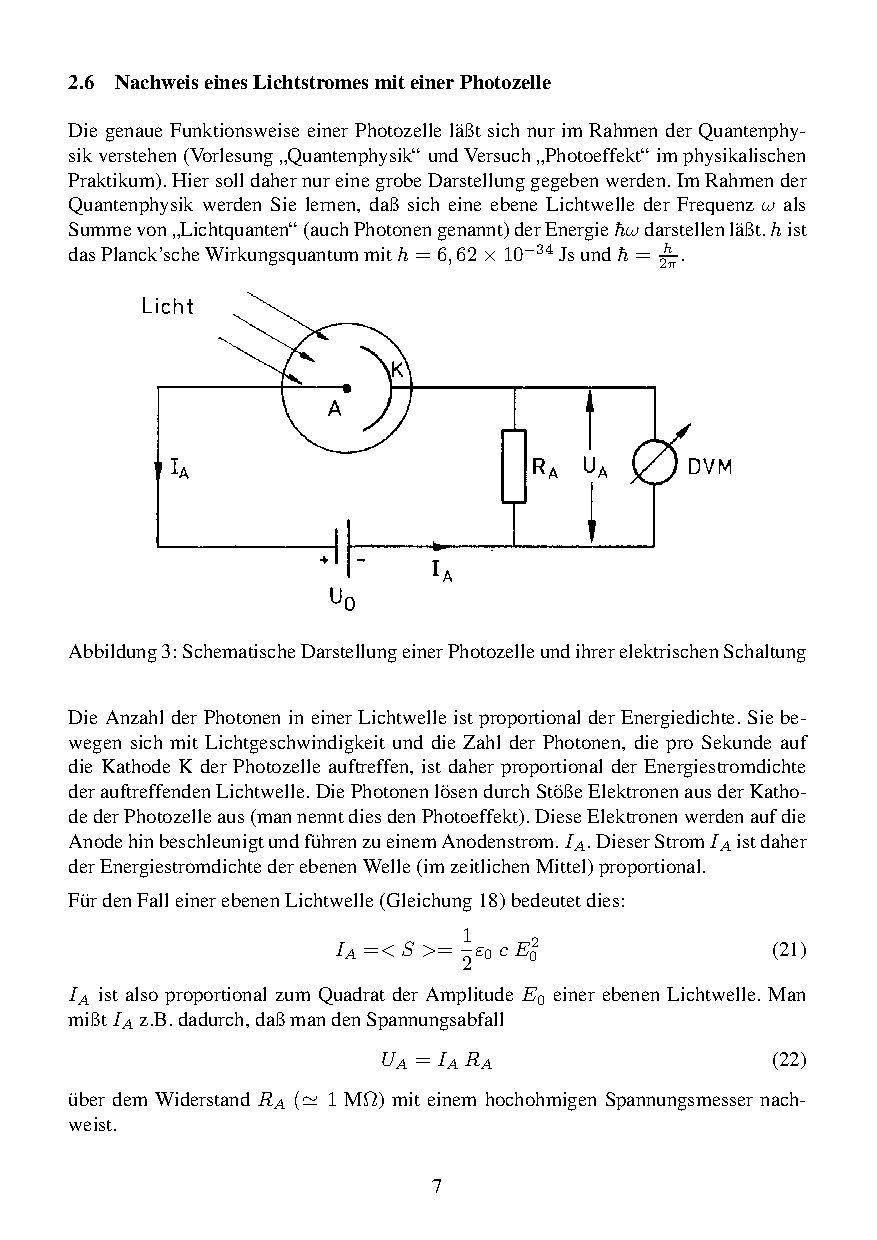
\includegraphics[trim = 0mm 112mm 0mm 50mm, clip, scale = 1]{abb_3.pdf}
  	\caption[Skizze der Photozelle]{Skizze der Photozelle\footnotemark}
  \label{fig:abb_3}
\end{figure}
\footnotetext{Abbildung entnommen von http://www.atlas.uni-wuppertal.de/~kind/wp1.pdf Seite 7 am 07.09.2014}

den Wert von 1,0$\mu$A nicht überschreitet. ($U_A \approx$ 70V, $R_A$ = 1M$\Omega$) Der Photostrom $I_A$ wird anschließend für verschiedene Winkel $\theta$ bestimmt um das Malussche Gesetz zu überprüfen.
Dafür stellen wir $I_A$ als Funktion von $\theta$ grafisch dar.
Zuletzt stellen wir einen dritten Polarisator zwischen die beiden anderen, deren Durchlaßrichtung
um 90$^\circ$ gegeneinander verdreht ist. Wir wollen den Winkel, bei dem der größte Anteil des Lichtes durchgelassen wird, bestimmen.
%Erklären Sie schriftlich Ihre Beobachtung.
\subsubsection{Theoretische Durchführung}
Nach dem Malusschen Gesetz ist der folgende Zusammenhang zu erwarten:
\begin{align}
I_A \propto <S> = \frac{1}{2} \varepsilon_0 c E'^2
\end{align}
$I_A$ der Anodenstrom, $S$ die Energieflussdichte und $E'$ die Amplitude der Lichtwelle hinter dem Polarisator.
Für $E'$ gilt:
\begin{align}
E' = E_0 \cos{\theta}
\end{align}
$E_0$ die Anfangsamplitude des Lichtes.\\
Schließlich Folgt:
\begin{align}
I_A \propto \cos^2{\theta}
\label{eqn:a_1}
\end{align}
\subsection{Messergebnisse}
\begin{table}[H]
\caption{Messdaten zur Verifikation des Mallusschen Gesetzes, wobei der Fehler des Winkels bei $(\pm 1)$ Grad  und der Fehler der Spannung bei $(\pm 0,1)$ V liegt. Der Widerstand hatte einen Wert von 1MOhm $(\pm 5$\%)}
\begin{center}
\begin{tabular}{|r|r|}
\hline
\multicolumn{1}{|l|}{Winkel/Grad} & \multicolumn{1}{l|}{Spannung/V} \\ \hline
0 & 0,99 \\ \hline
5 & 0,98 \\ \hline
10 & 0,95 \\ \hline
15 & 0,92 \\ \hline
20 & 0,85 \\ \hline
25 & 0,78 \\ \hline
30 & 0,71 \\ \hline
35 & 0,63 \\ \hline
40 & 0,54 \\ \hline
45 & 0,45 \\ \hline
50 & 0,36 \\ \hline
55 & 0,27 \\ \hline
60 & 0,19 \\ \hline
65 & 0,13 \\ \hline
70 & 0,07 \\ \hline
75 & 0,04 \\ \hline
80 & 0,02 \\ \hline
85 & 0,01 \\ \hline
90 & 0,01 \\ \hline
\end{tabular}
\end{center}
\label{tab:a_1}
\end{table}
\subsection{Auswertung}
In der ersten Aufgabe sollte das Mallussche Gesetz verifiziert werden. Dazu wurde der Photostrom in Abhängigkeit vom Winkel des zweiten Polarisators in Bezug zum ersten gemessen. Es ergab sich der folgende Plot (Werte aus Tabelle \ref{tab:a_1}).

\begin{figure}[H]
\centering
    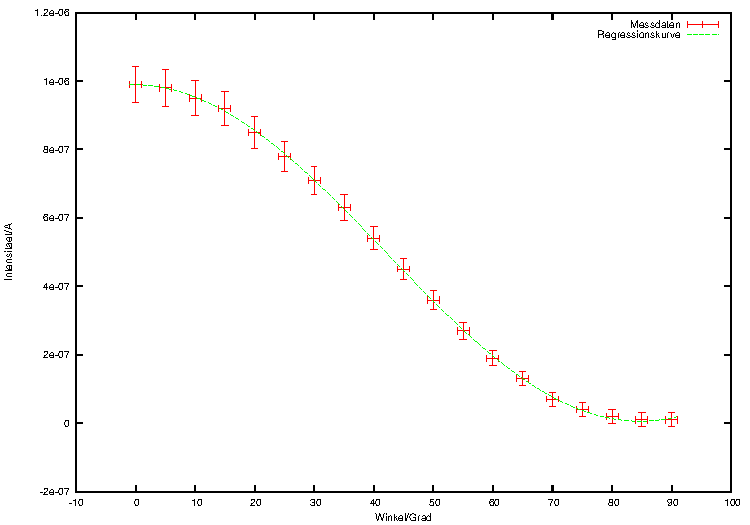
\includegraphics[scale = 1]{a_1.pdf}
  	\caption[Plot der Intensität in Abhängigkeit des Winkels]{Plot der Intensität in Abhängigkeit des Winkels}
  \label{fig:a_1}
\end{figure}

Die Messdaten wurden dabei nach Gleichung \ref{eqn:a_1} gefittet. Es ergaben sich die folgende Fitparameter I($\phi$) = -9.83414e-07 $(\pm 5.092e-09) \cdot$ cos$^2(\phi \cdot$ 0.0184 $(\pm 0.0002)$ + 1.580 $(\pm 0.009) )$ + 9.89381e-07 $(\pm 4.11e-09)$.

Dann sollte ein dritter Polarisator zwischen die ersten beiden gestellt, und überprüft werden, wann die Intensität maximal wird. Dabei ergab sich ein Wert von (45 $\pm 2)$Grad. Bei einem Winkel von $\pm$90 Grad ist keine Intensität mehr zu messen.
\subsection{Diskussion}
Das Ergebnis der ersten Aufgabe ist gut an der Regression (Abbildung \ref{fig:a_1}) zu erkennen, welche auf nahezu allen Messpunkten aufliegt.


\section{Versuch WO1.2: Beobachtung der Polarisation von Licht durch Einfachstreuung}
\subsection{Versuchsdurchführung}

\begin{figure}[H]
\centering
    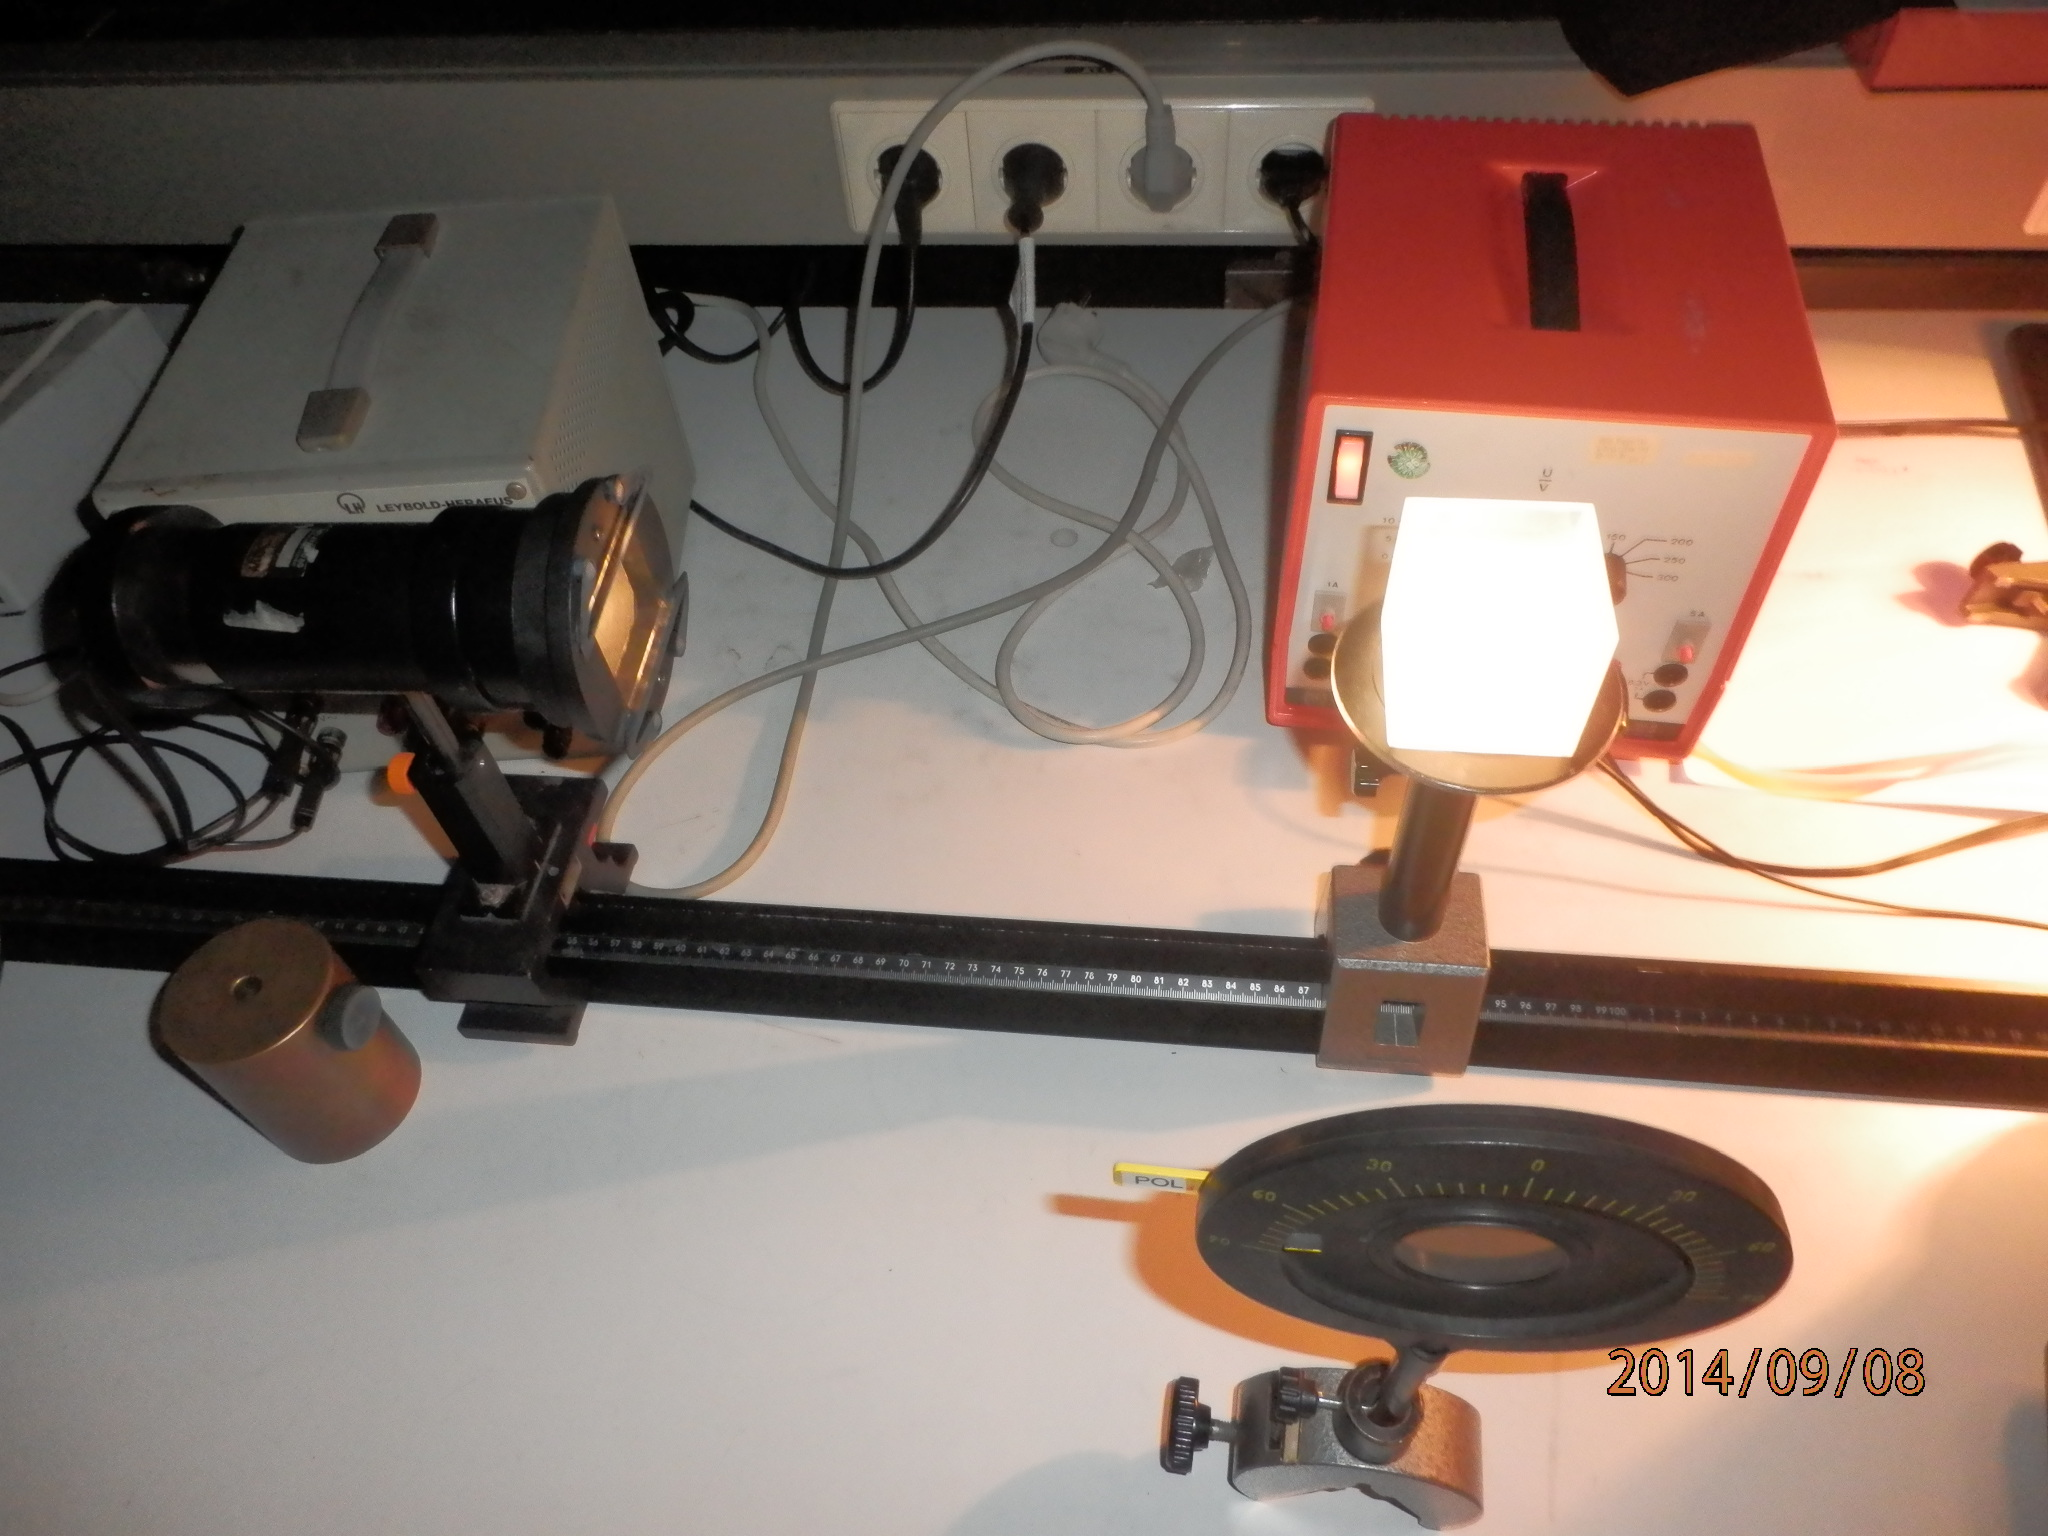
\includegraphics[scale = 0.1]{aufgabe_2.JPG}
  	\caption[Foto des Versuchsaufbaus der zweiten Aufgabe]{Foto des Versuchsaufbaus der zweiten Aufgabe}
  \label{fig:aufgabe_2}
\end{figure}

\subsubsection{Praktische Durchführung}
Wir bauen auf einer optischen Bank den in der Folgenden Abbildung skizzierten
Versuch auf.
%Bitte Abbildung 10 aus der Versuchsbeschreibung einfügen

\begin{figure}[H] 
  \centering
    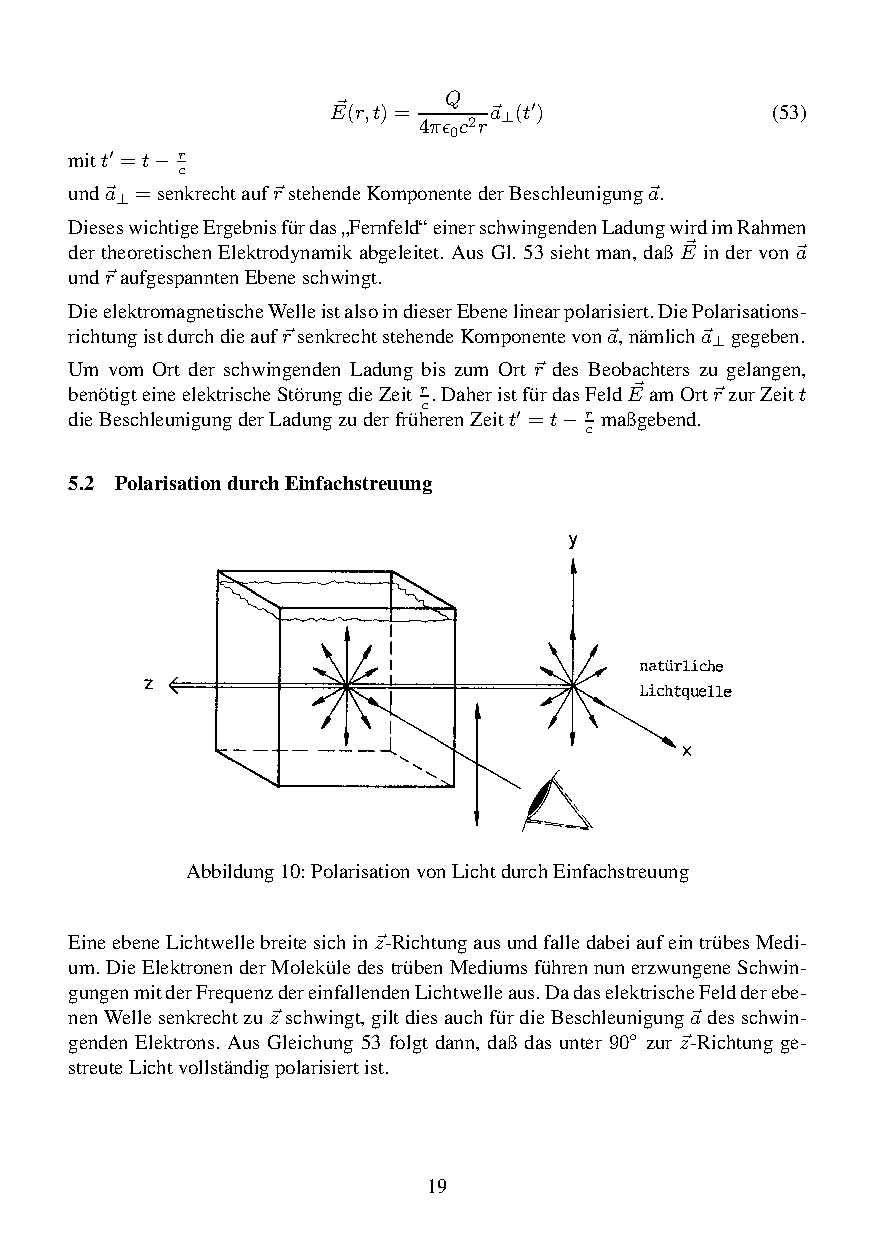
\includegraphics[trim = 0mm 65mm 0mm 90mm, clip, scale = 1]{abb_10.pdf}
  	\caption[Skizze der Photozelle]{Skizze der Photozelle\footnotemark}
  \label{fig:abb_10}
\end{figure}
\footnotetext{Abbildung entnommen von http://www.atlas.uni-wuppertal.de/~kind/wp1.pdf Seite 19 am 07.09.2014}

Als Lichtquelle dient eine Glühlampe mit Kondensor. Das von dieser Lichtquelle ausgehende Lichtbündel fällt auf eine wässrige Lösung von Styrofan in einer rechteckigen Glasküvette.
Wir sehen uns das unter
90$^\circ$ gestreute Licht durch einen Polarisationsfilter (= Analysator) an. 
%Was beobachten Sie bei Drehung des Analysators? Ist das Streulicht polarisiert? Wenn ja, in welche Richtung? Ist die Polarisation vollständig?
\subsection{Auswertung}
In der zweiten Aufgabe sollte der bei einer Styrofanlösung senkrecht abgestrahlte Teil des Lichts mit einem Polarisator untersucht werden. Bei der Drehung des Polarisators war eine Intensitätsab- bzw. zunahme, so wie eine Verschiebung des Lichtspektrums zu beobachten. Die minimale Intensität erhielten wir bei einer Drehung von 90 Grad, die maximale Intensität haben wir bei 0 Grad gemessen. Aus den Beobachtungen lässt sich schließen, dass das Licht zum Teil polarisiert war, da bei minimaler Intensität weiterhin ein Teil des Lichtes durchgelassen wurde.
\subsection{Diskussion}
In der zweiten Aufgabe war zwar eine Abschwächung der Intensität zu beobachten, sowie eine Verschiebung des Farbspektrums, jedoch konnte keine vollständige Polarisation des Lichtes bestätigt werden. Dies liegt warscheinlich daran, dass die Verdünnung unserer Styrofanlösung einerseits nicht hoch genug war, sodass neben dem Polarisationseffekt z.B. Streueffekte eine große Rolle spielten, und andererseits die Ausbreitungsrichtung des Lichtes schon durch die Glühlampe stark variierte und wir dadurch nicht senkrecht zu den Aubreitungsrichtungen aller "Lichtstrahlen" beobachten konnten. 


\section{Versuch WO1.3:
Messung der Richtungscharakteristik der Strahlung einer schwingenden Ladung}
\subsection{Versuchsdurchführung}

\begin{figure}[H]
\centering
    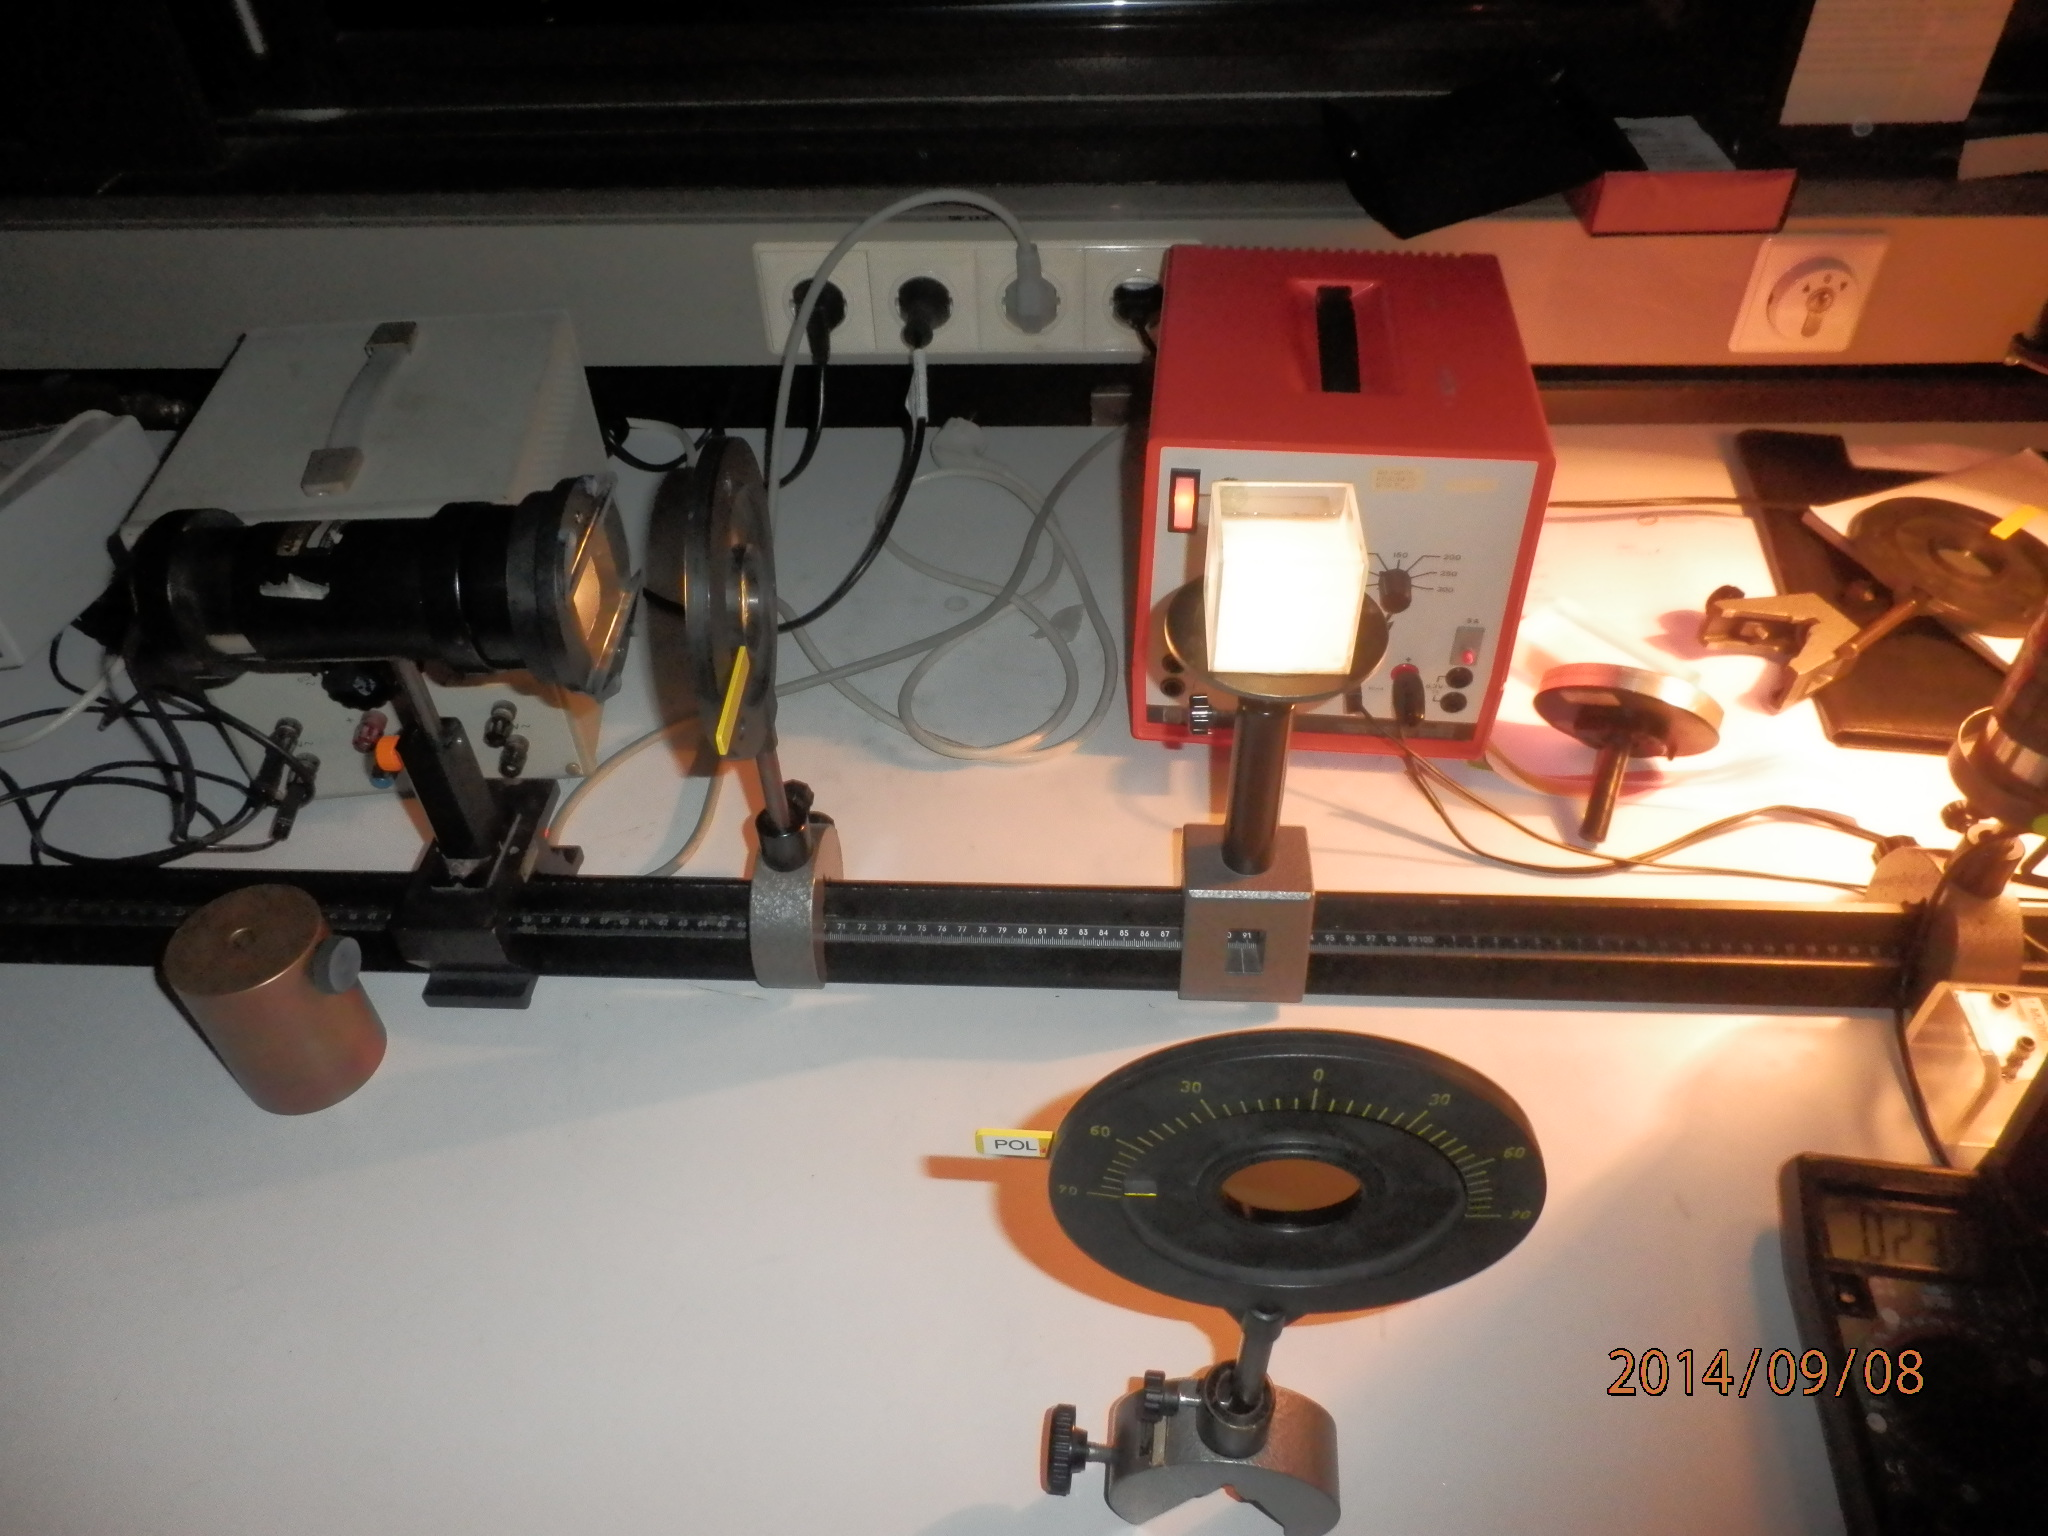
\includegraphics[scale = 0.1]{aufgabe_3.JPG}
  	\caption[Foto des Versuchsaufbaus der dritten Aufgabe]{Foto des Versuchsaufbaus der dritten Aufgabe}
  \label{fig:aufgabe_3}
\end{figure}

\subsubsection{Praktische Durchführung}
Wir verwenden den Versuchsaufbau zu Versuch WO1.2, um den in der folgenden Abbildung skizzierten Aufbau zu realisieren (lediglich der Polarisationsfilter wechselt seinen Platz).
%Bitte Abbildung 11 aus der Versuchsbeschreibung einfügen

\begin{figure}[H] 
  \centering
    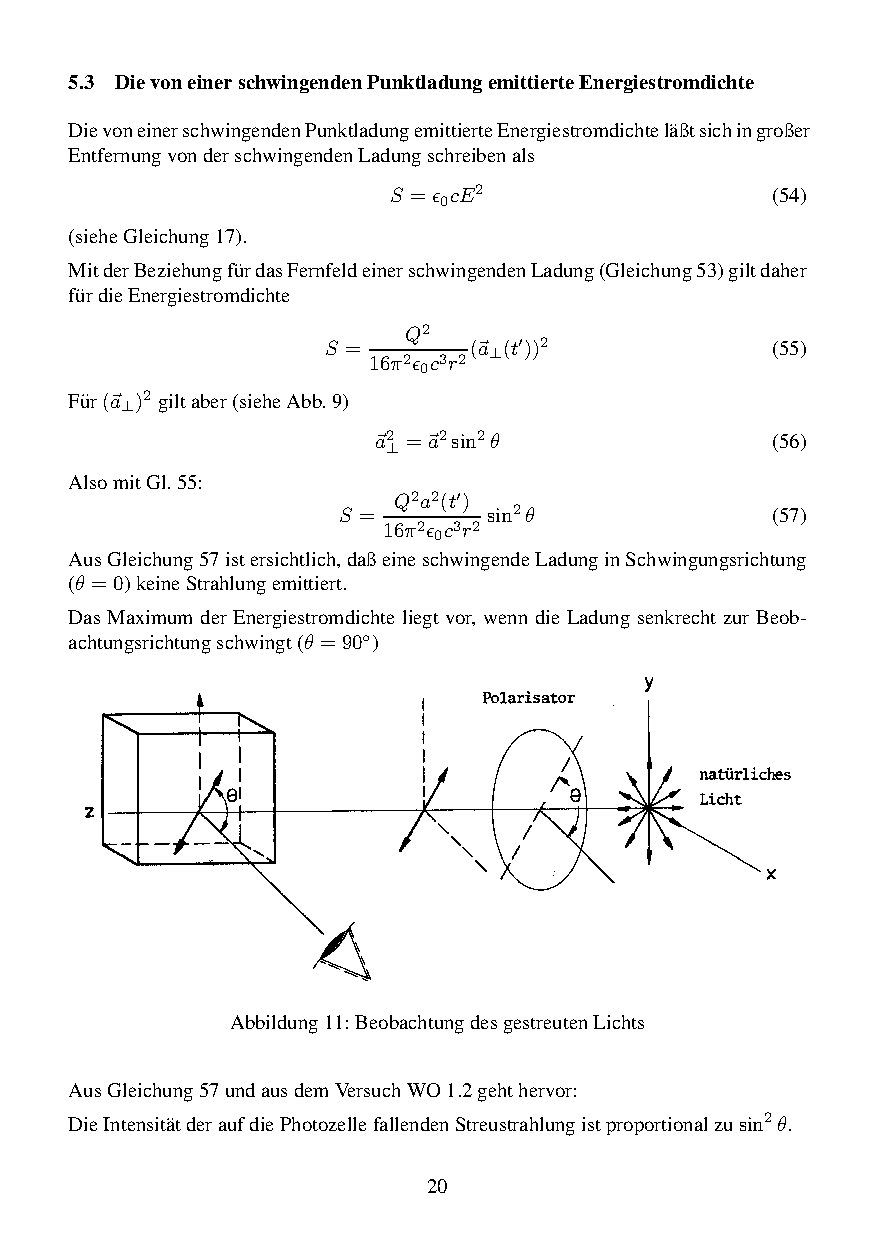
\includegraphics[trim = 0mm 40mm 0mm 113mm, clip, scale = 1]{abb_11.pdf}
  	\caption[Skizze der Photozelle]{Skizze der Photozelle\footnotemark}
  \label{fig:abb_11}
\end{figure}
\footnotetext{Abbildung entnommen von http://www.atlas.uni-wuppertal.de/~kind/wp1.pdf Seite 20 am 07.09.2014}

Wir drehen den Polarisationsfilter anschließend und beobachten den Intensitätsunterschied.
\subsection{Auswertung}
In der dritten Aufgabe sollte der selbe Aufbau wie zuvor verwendet werden. Es sollte jedoch ein Polarisator zwischen Styrofanlösung und Strahler gestellt werden. Dabei ergaben sich bei 0 Grad die selben Ergebnisse wie in Aufgabe 2. Bei Drehung des Polarisators um 90 Grad blieb die Intensität des beobachteten Lichtes nahezu gleich (sie war bei 0 Grad sogar etwas größer, als bei 90 Grad).
\subsection{Diskussion}
Bei dem Ergebnis des dritten Aufgabe verhält es sich wie bei der zweiten Aufgabe, da wir die selbe Lösung wie vorher verwendet haben sowie die selbe Lampe zur Beleuchtung. Trotzdem konnte der erwartete Effekt bestätigt werden (,das austretende Licht war stärker für eine Polarisation des eingestrahlten Lichtes senkrecht zur Beobachtungs- und Ausbreitungsrichtung).

\section{Versuch WO1.4:
Das Brewstersche Gesetz}
\subsection{Versuchsdurchführung}

\begin{figure}[H]
\centering
    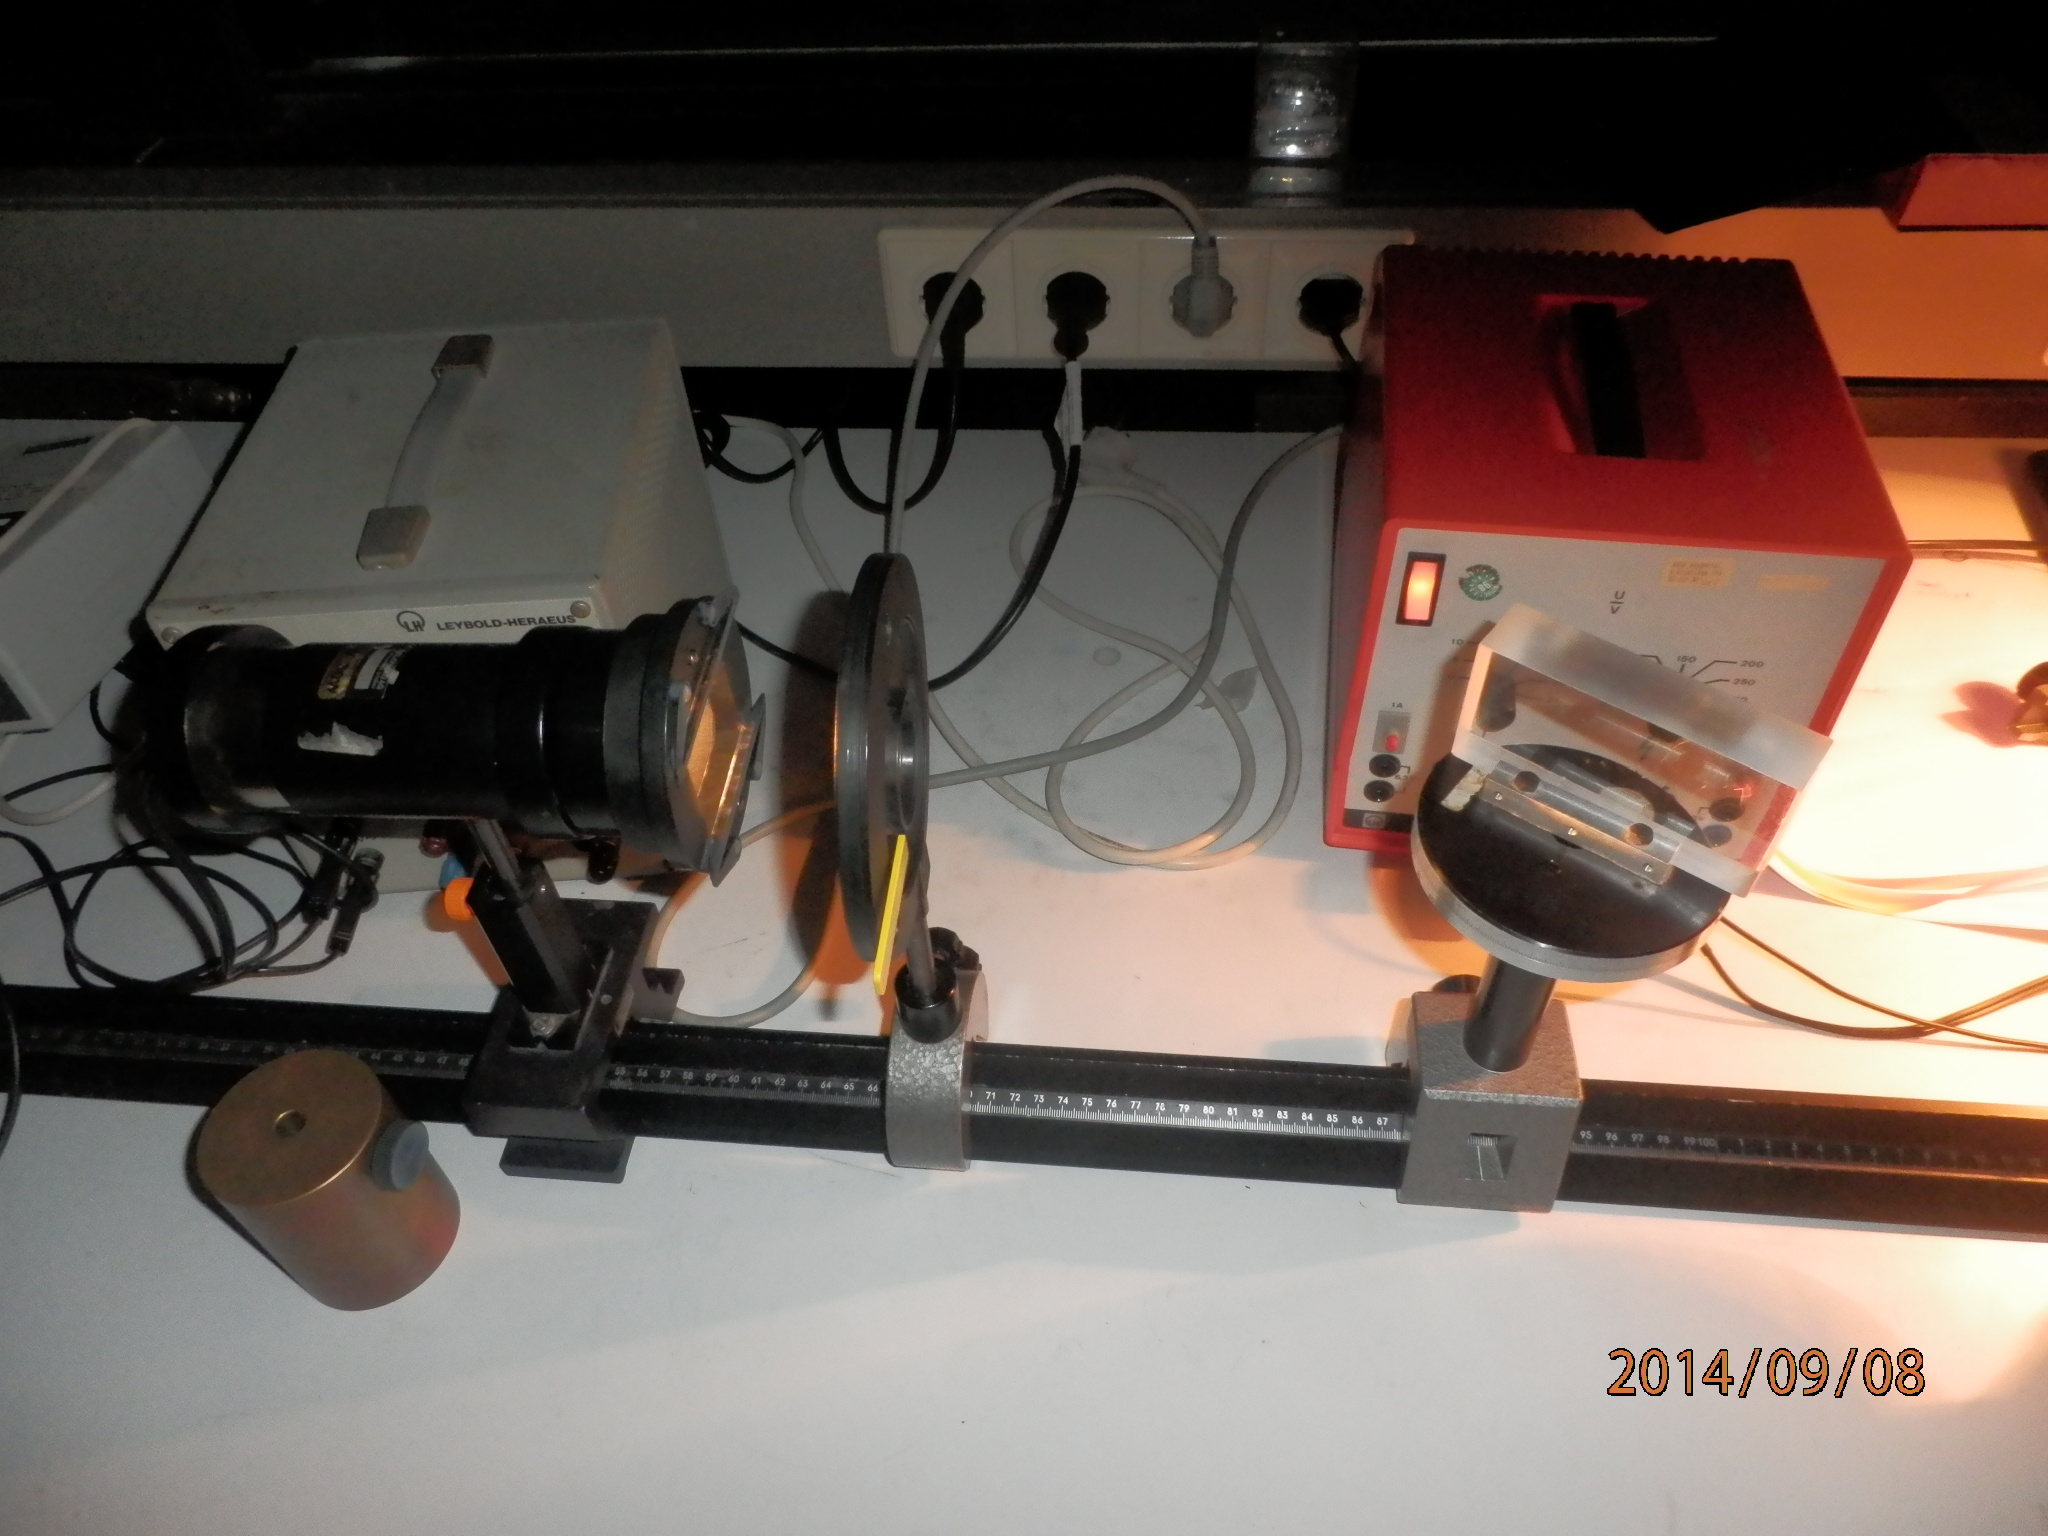
\includegraphics[scale = 0.1]{aufgabe_4.JPG}
  	\caption[Foto des Versuchsaufbaus für die vierte Aufgabe]{Foto des Versuchsaufbaus für die vierte Aufgabe}
  \label{fig:aufgabe_4}
\end{figure}

\subsubsection{Praktische Durchführung}
Wir verifizieren das sogenannte Brewstersche Gesetz experimentell, indem wir im Ver-
suchsaufbau zu WO1.2 die Glasküvette durch einen Glasblock (Plexiglas) ersetzen und
die Polarisation des reflektierten Lichtes beobachten.
Der Glasblock wird dabei auf einen Drehtisch mit Winkelskala gesetzt.
%Auf dem Tisch ist eine Schiene, an die der Block angelegt wird, damit eine feste Beziehung zwischen Drehtischskala und Glasoberfläche entsteht. Die Winkelskala kann leicht verdreht sein. (Können Sie diesen Fehler kompensieren, wenn Sie den Brewsterwinkel nach beiden Seiten hin messen?) Aus den Betrachtungen zu den Versuchen WO1.2 und WO1.3 können Sie die Gültigkeit des Brewsterschen Gesetzes verstehen. 
Bei dieser Messung ist zu beachten, dass der reflektierte Strahl von ”schwingenden Glasmolekülen“ ausgesandt wird, welche in einer Ebene
senkrecht zur Ausbreitungsrichtung des gebrochenen Strahls schwingen.
Ziel ist es den Winkel zu bestimmen, bei dem das Licht nahezu vollständig polarisiert ist.(Brewsterwinkel)
%Am sichersten ist es zu beobachten, wann nahezu kein reflektiertes Licht mehr durch den (um 90$^\circ$verdrehten) Analysator gelangt.
Aus dem Brewsterwinkel wird dann %nach Gleichung \ref{}
der Brechungsindex berechnet.
\subsubsection{Theoretische Durchführung}
Für den Brewsterwinkel gilt die Beziehung:
\begin{align}
\tan{\theta} = n_G
\label{eqn:a_2}
\end{align}
$n_G$ ist der Brechungsindex von Plexiglas.\\
Der Fehler für den Brewsterwinkel ist:
\begin{align}
\sigma_\theta = (1+\tan^2{n_G})\sigma_{n_G}
\label{eqn:a_2_sigma}
\end{align}
\subsection{Messergebnisse}
\begin{table}[htbp]
\caption{Messdaten zur bestimmung des Brechungsindex, mit den Brewstonschen Winkel.}
\begin{center}
\begin{tabular}{|l|l|}
\hline
Winkel/Grad & Fehler/Grad \\ \hline
\multicolumn{1}{|r|}{56} & \multicolumn{1}{r|}{2} \\ \hline
\end{tabular}
\end{center}
\label{tab:a_4}
\end{table}
\subsection{Auswertung}
In der vierten Aufgabe sollte mit Hilfe des Brewsterwinkels der Brechungsindex von Plexiglas bestimmt werden. Wir haben einen Winkel von 56 $(\pm 2)$ Grad gemessen. Damit wurde nach Gleichung \ref{eqn:a_2} ein Brechungsindex und nach Gleichung \ref{eqn:a_2_sigma} der Fehler bestimmt. Es ergab sich ein Wert von 1,48 $(\pm3,58)$.
\subsection{Diskussion}
Der bestimmte Brechungsindex von 1,48 ist bei einem Literaturwert von 1,46 akzeptabel, da dieser innerhalb des Fehlerbalkens des gemessenen Wertes liegt, welcher ein prozentualen Anteil von etwas mehr als 7,5 \% am Messwert hat.

\section{Versuch WO2.1:
Doppelbrechung von Cellophan}
\subsection{Versuchsdurchführung}

\begin{figure}[H]
\centering
    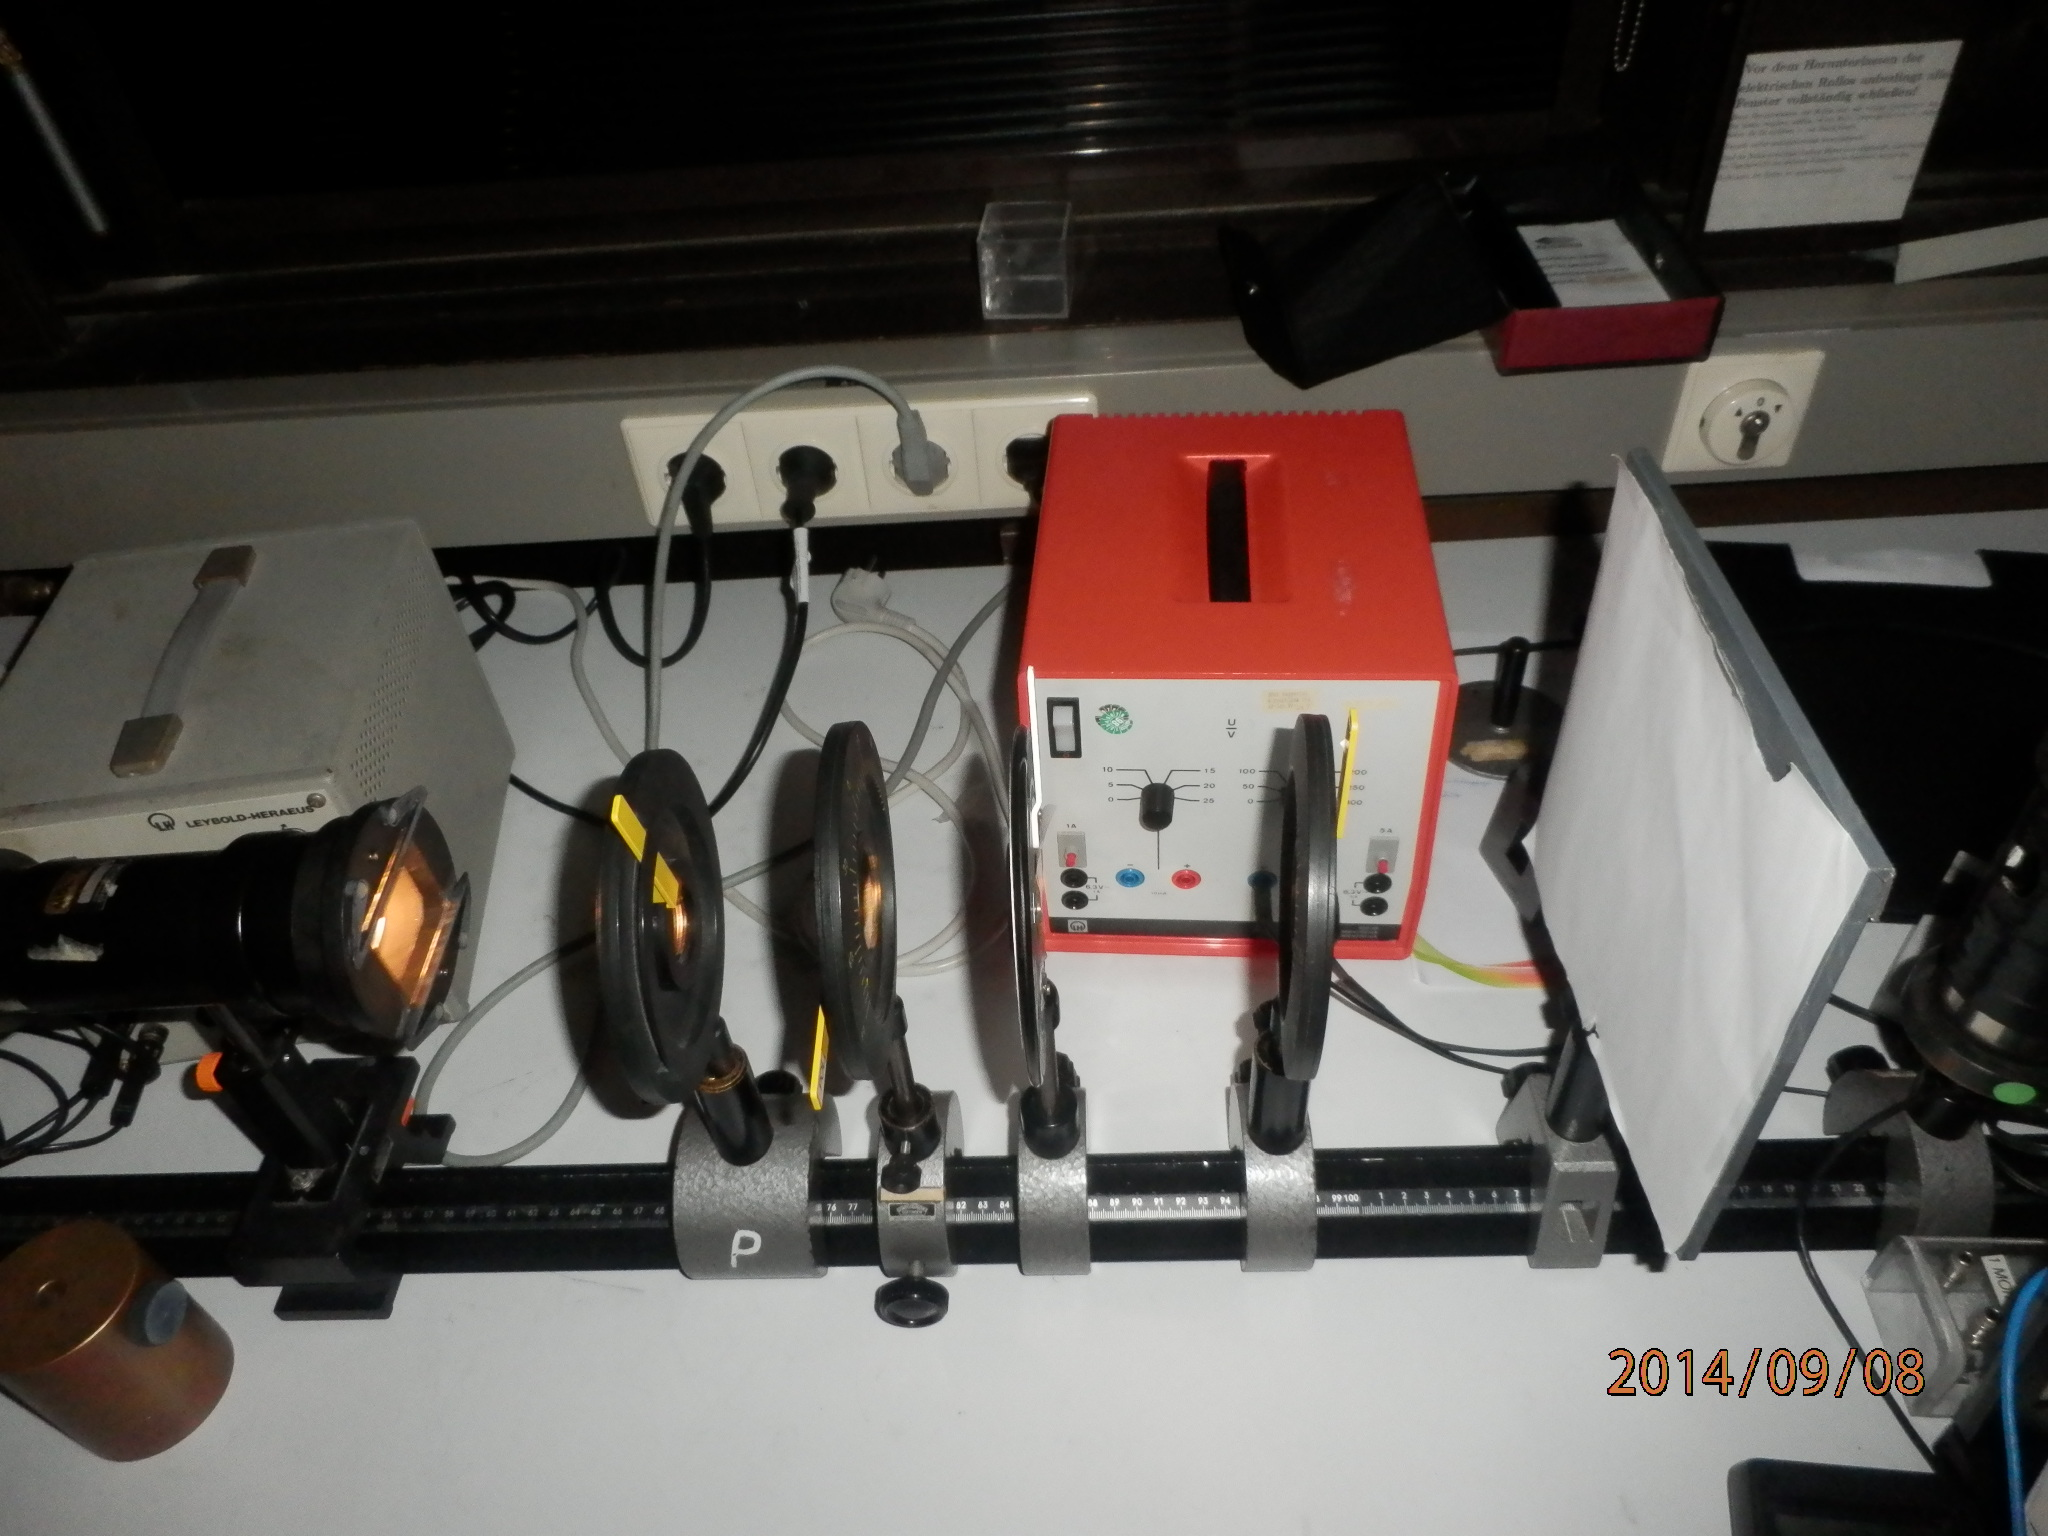
\includegraphics[scale = 0.1]{aufgabe_5_1.JPG}
  	\caption[Foto des Versuchsaufbaus der fünften Aufgabe mit PVP]{Foto des Versuchsaufbaus der fünften Aufgabe mit PVP}
  \label{fig:aufgabe_5_1}
\end{figure}

\begin{figure}[H]
\centering
    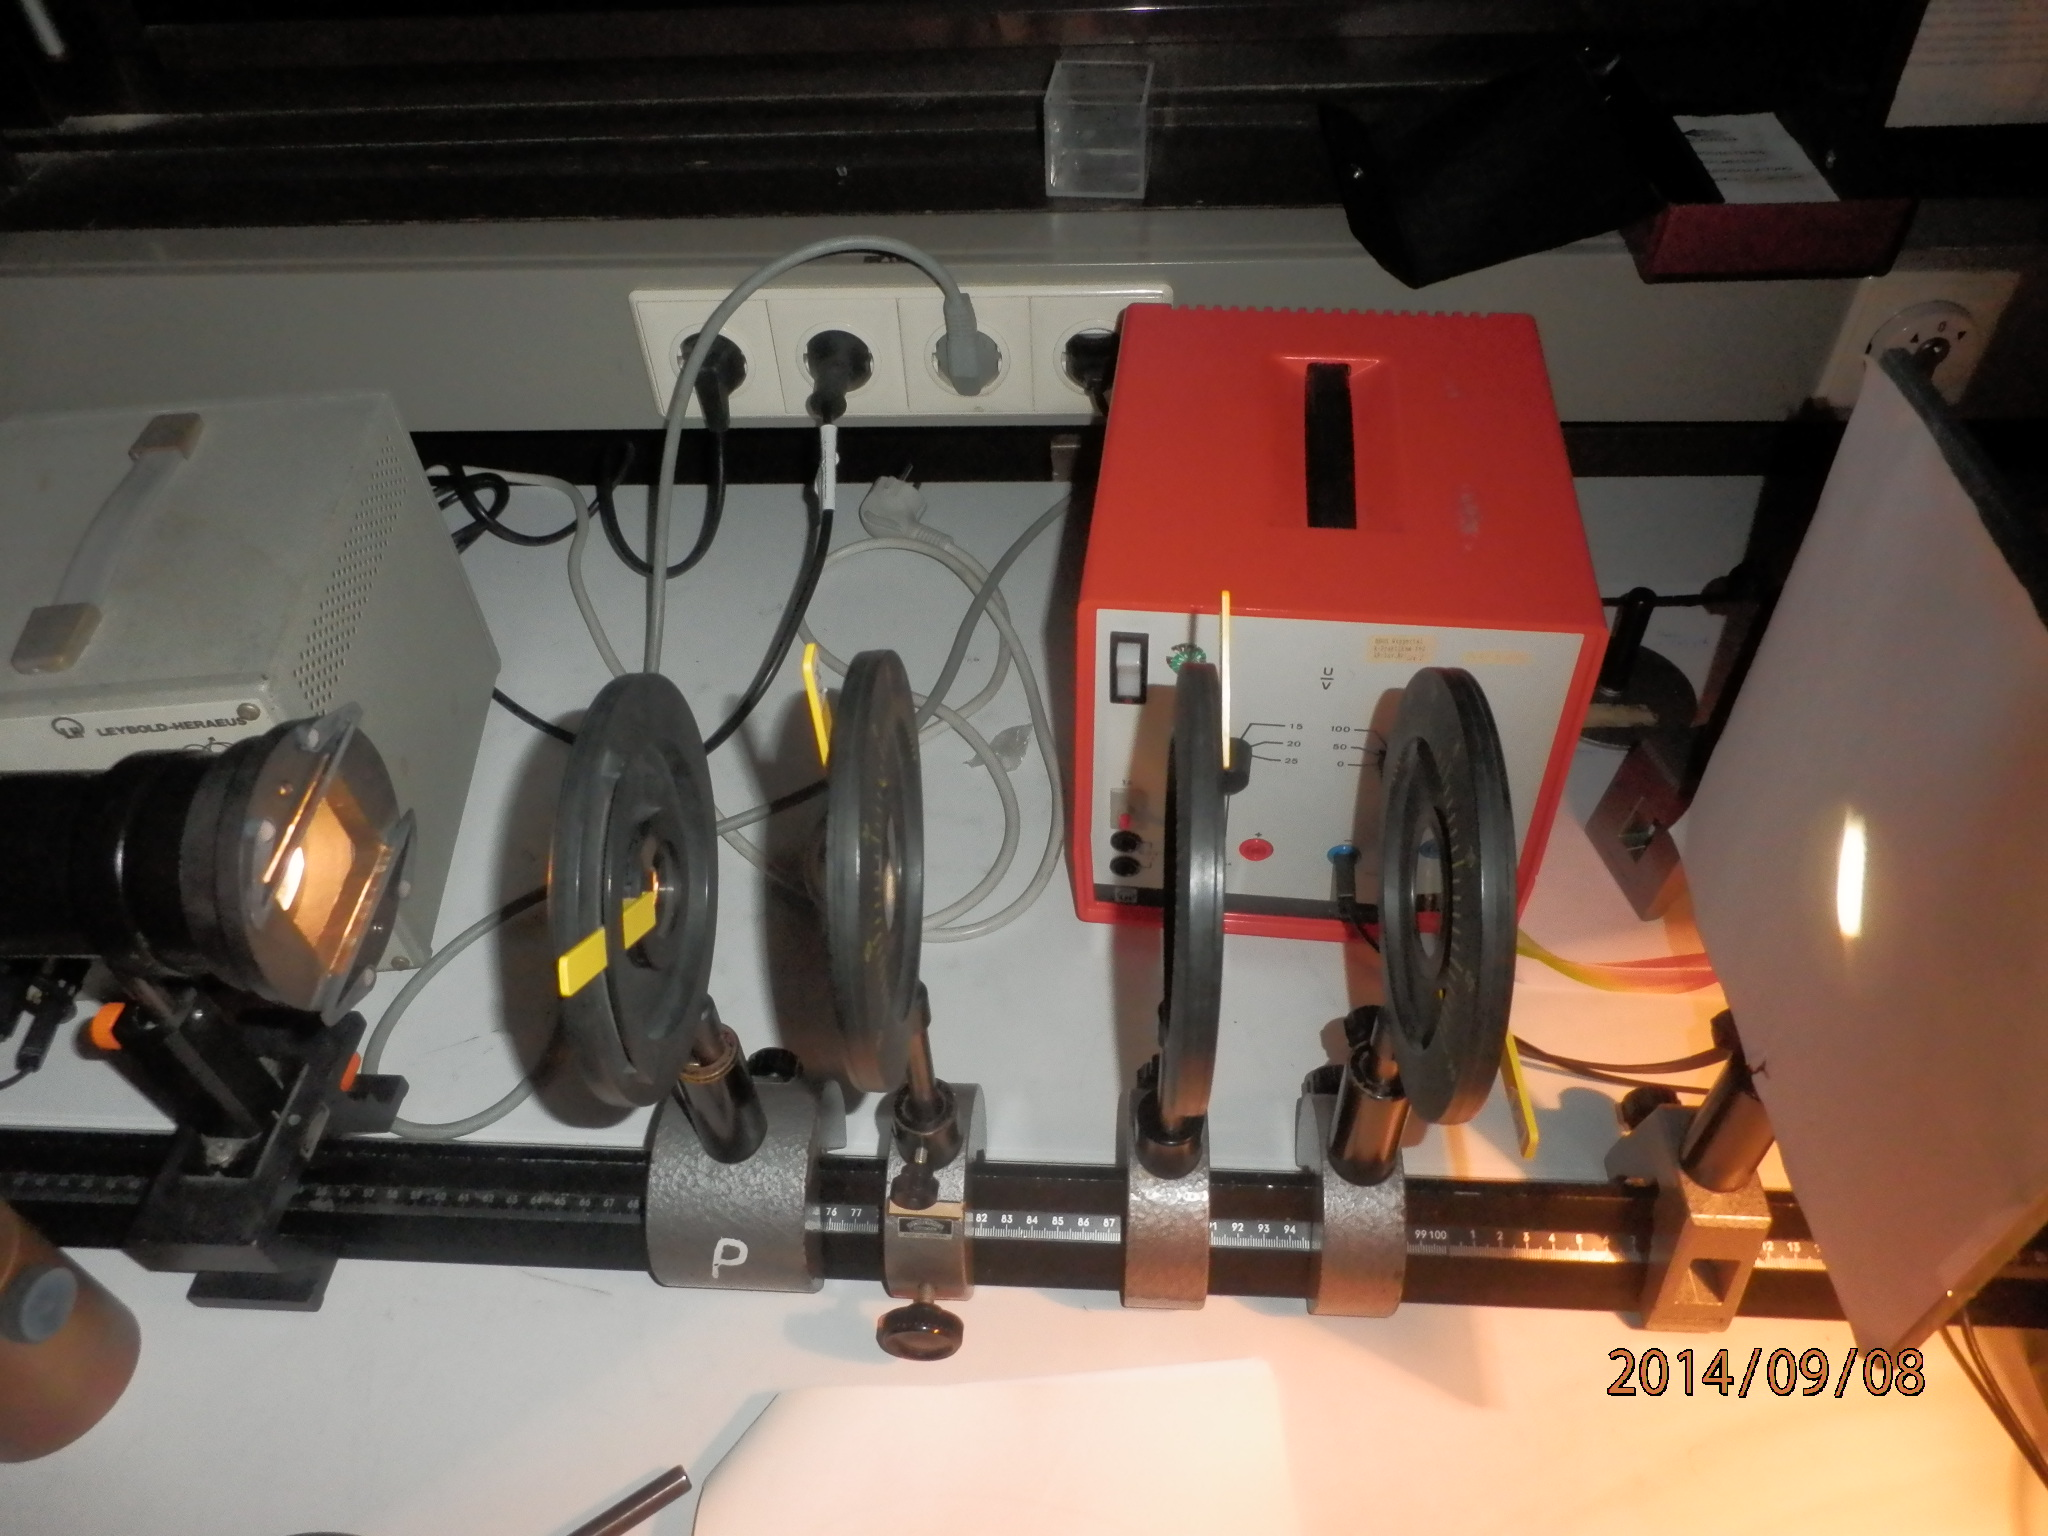
\includegraphics[scale = 0.1]{aufgabe_5_2.JPG}
  	\caption[Foto des Versuchsaufbaus der fünften Aufgabe, mit einem $\frac{\lambda}{4}$-Plättchen]{Foto des Versuchsaufbaus der fünften Aufgabe, mit einem $\frac{\lambda}{4}$-Plättchen}
  \label{fig:aufgabe_2}
\end{figure}

\subsubsection{Praktische Durchführung}
\begin{enumerate}
\item[a)]
Wir stellen aus einer Dreh- oder Spannhalterung und einem Stück Cellophanfolie (Klebefolie, Verpackungsfolie) ein Phasenverschiebungsplättchen (PVP) her. %(nur 1 Folie!).
Die Wirkung des PVP, die wir bei Drehung des PVP zwischen zwei gekreuzten Polaroidfiltern beoachten, soll untersucht und die Lage der optischen Achsen bestimmt werden.
%(in gleicher Halterung wie die Polarisationsfilter). Bitte verwechseln sie die Plättchen nicht mit den Filtern! Sie können die $\frac{\lamda}{4}$-Plättchen an zwei Merkmalen von den Polarisationsfiltern unterscheiden: 1) Polarisationsfilter lassen nur die Hälfte des natürlichen Lichtes durch und sind daher dunkelgrau, $\frac{\lambda}{4}$-Plättchen hingegen klar transparent. 2) Die Fassung der $\frac{\lambda}{4}$-Plättchen trägt den Aufdruck ”$\frac{\lambda}{4}$“. Die Polarisationsfilter sind unbeschriftet. 3) Keine Rolle spielt die Farbe der Drehhebel oder Aufschrift (weiß oder gelb)!
\item[b)] Wir Nehmen nun ein industrielles
$\frac{\lambda}{4}$-Plättchen und drehen es so, dass der Polarisator genau zwischen den beiden optischen Achsen (45$^\circ$) des $\frac{\lambda}{4}$-Plättchens steht.
Wir variieren die Durchlassrichtung des Analysators und beobachten Intensitäts- und Farbeffekte für das weiße Glühlampenlicht und für die fünf
Farbfilter (violett, blau, grün, gelb und rot). Die Monochromfilter 
%(achten Sie auf die fünfstellige Nummer am Filterrahmen und nicht nur auf die Filterfarbe!)
haben folgende Durchlässigkeitsbereiche (DLB) für die Wellenlänge:
%bitte Abbildung aus der Versuchsanleitung einfügen

%Für welche Farbe weist Ihr$\frac{\lambda}{4}$-Plättchen annähernd die Eigenschaften eines idealen $\frac{\lambda}{4}$-Plättchens auf ?
\item[c)] Wir haben elliptisch polarisiertes Licht hergestellt und wollen untersuchen, ob sich die Lage der Ellipse ändert, wenn wir das $\frac{\lambda}{4}$-Plättchen um 90$^\circ$
drehen. Später vergleichen wir unsere Beobachtung mit der theoretischen Erwartung.
\item[d)] Nach den Ergebnissen aus b) können wir für einen Farbfilter mit Hilfe des $\frac{\lambda}{4}$-Plättchens nahezu einen Zirkularpolarisator (ZP) herstellen, und zwar sowohl links- als auch rechtsdrehend. Wir stellen zwei ZP her und beobachten die Intensitätsverteilung bei verschiedenen Winkelstellungen zwischen den Durchlassrichtungen der beiden Polaroidfilter und den optischen Achsen der $\frac{\lambda}{4}$-Plättchen.
\end{enumerate}
\subsubsection{Theoretische Durchführung}
\begin{enumerate}
\item[a)]
Die optischen Achsen sind die Winkel, bei denen kein Licht durch den Aufbau gelangt, da das Licht einerseits nicht durch das PVP polarisiert wird und andererseits die beiden Polarisator um 90$^\circ$ zueinander verdreht sind.
\item[b)]
Wir erwarten für eine Farbe zirkular polarisiertes Licht.
Die Phasenverschiebung $\phi$ lässt sich berechnen durch:
\begin{align}
\phi = cos^{-1}\left(\frac{I_{max}-I_{min}}{I_{max}+I_{min}}\right)
\label{eqn:a_5_b}
\end{align}
Dabei können anstelle von $I$ auch zu $I$ proportionale Größen wie Strom oder Spannung verwendet werden.
Der Fehler ist:
\begin{align}
\sigma_{\phi} = \sqrt{
\left(\frac{\frac{2I_{max}}{(I_{max}+I_{min})^2}}{\sqrt{1-\left(\frac{I_{max}-I_{min}}{I_{max}+
I_{min}}\right)^2}}\sigma_{I_{min}}\right)^2+
\left(\frac{\frac{2I_{min}}{(I_{max}+I_{min})^2}}{\sqrt{1-\left(\frac{I_{max}-I_{min}}{I_{max}+
I_{min}}\right)^2}}\sigma_{I_{max}}\right)^2}
\label{eqn:a_5_b_sigma}
\end{align}
\item[c)]
Wir erwarten, dass sich die Polarisationsrichtung der Ellipse ändert, wobei die Lage der Ellipse gleich bleibt.
\item[d)]
Da wir beide ZP ($\frac{\lambda}{4}$-Plättchen um 90$^\circ$ verschoben) hintereinander geschaltet haben erwarten wir linear polarisiertes Licht.
\end{enumerate}
\subsection{Messergebnisse}
\begin{enumerate}
\item[b)]

\begin{table}[htbp]
\caption{Messdaten für weißes Licht. Der Fehler des Winkel wurde mit $(\pm 1)$Grad und der Fehler der Spannung mit $(\pm 0,1)$mV angenommen.}
\begin{center}
\begin{tabular}{|r|r|}
\hline
\multicolumn{1}{|l|}{Winkel/Grad} & \multicolumn{1}{l|}{Intensität/mV} \\ \hline
0 & 24,55 \\ \hline
20 & 26 \\ \hline
40 & 26,7 \\ \hline
60 & 26,8 \\ \hline
80 & 25,7 \\ \hline
100 & 24,1 \\ \hline
120 & 22,7 \\ \hline
140 & 22,3 \\ \hline
160 & 23,1 \\ \hline
180 & 24,2 \\ \hline
\end{tabular}
\end{center}
\label{tab:a_5_b_w}
\end{table}


\begin{table}[htbp]
\caption{Messdaten für dunkelrotes Licht. Der Fehler des Winkel wurde mit $(\pm 1)$ und der Fehler der Spannung mit $(\pm 0,1)$ mV angenommen.}
\begin{center}
\begin{tabular}{|r|r|}
\hline
\multicolumn{1}{|l|}{Winkel/Grad} & \multicolumn{1}{l|}{Intensität/mV} \\ \hline
0 & 7,6 \\ \hline
20 & 8,55 \\ \hline
40 & 9,7 \\ \hline
60 & 10,7 \\ \hline
80 & 11 \\ \hline
100 & 10,4 \\ \hline
120 & 9,2 \\ \hline
140 & 8 \\ \hline
160 & 7,4 \\ \hline
180 & 7,4 \\ \hline
\end{tabular}
\end{center}
\label{tab:a_5_b_dr}
\end{table}

\begin{table}[htbp]
\caption{Messdaten für gelbes Licht. Der Fehler des Winkel wurde mit $(\pm 1)$ und der Fehler der Spannung mit $(\pm 0,1)$ mV angenommen.}
\begin{center}
\begin{tabular}{|r|r|}
\hline
\multicolumn{1}{|l|}{Winkel/Grad} & \multicolumn{1}{l|}{Intensität/mV} \\ \hline
0 & 3,3 \\ \hline
20 & 3,5 \\ \hline
40 & 3,7 \\ \hline
60 & 3,8 \\ \hline
80 & 3,6 \\ \hline
100 & 3,4 \\ \hline
120 & 3,2 \\ \hline
140 & 3,2 \\ \hline
160 & 3,2 \\ \hline
180 & 3,5 \\ \hline
\end{tabular}
\end{center}
\label{tab:a_5_b_g}
\end{table}

\begin{table}[htbp]
\caption{Messdaten für gelbgrünes Licht. Der Fehler des Winkel wurde mit $(\pm 1)$ und der Fehler der Spannung mit $(\pm 0,1)$ mV angenommen.}
\begin{center}
\begin{tabular}{|r|r|}
\hline
\multicolumn{1}{|l|}{Winkel/Grad} & \multicolumn{1}{l|}{Intensität/mV} \\ \hline
0 & 6,6 \\ \hline
20 & 6,65 \\ \hline
40 & 6,15 \\ \hline
60 & 5,25 \\ \hline
80 & 4,35 \\ \hline
100 & 3,9 \\ \hline
120 & 4,1 \\ \hline
140 & 4,9 \\ \hline
160 & 5,8 \\ \hline
180 & 6,4 \\ \hline
\end{tabular}
\end{center}
\label{tab:a_5_b_gg}
\end{table}

\begin{table}[htbp]
\caption{Messdaten für blaugrünes Licht. Der Fehler des Winkel wurde mit $(\pm 1)$ und der Fehler der Spannung mit $(\pm 0,1)$ mV angenommen.}
\begin{center}
\begin{tabular}{|r|r|}
\hline
\multicolumn{1}{|l|}{Winkel/Grad} & \multicolumn{1}{l|}{Intensität/mV} \\ \hline
0 & 55,8 \\ \hline
20 & 60,7 \\ \hline
40 & 66,4 \\ \hline
60 & 71,8 \\ \hline
80 & 72,9 \\ \hline
100 & 69,4 \\ \hline
120 & 63,1 \\ \hline
140 & 56,95 \\ \hline
160 & 54,2 \\ \hline
180 & 55,8 \\ \hline
\end{tabular}
\end{center}
\label{tab:a_5_b_bg}
\end{table}

\begin{table}[htbp]
\caption{Messdaten für violettes Licht. Der Fehler des Winkel wurde mit $(\pm 1)$ und der Fehler der Spannung mit $(\pm 0,1)$ mV angenommen.}
\begin{center}
\begin{tabular}{|r|r|}
\hline
\multicolumn{1}{|l|}{Winkel/Grad} & \multicolumn{1}{l|}{Intensität/V} \\ \hline
0 & 8,9 \\ \hline
20 & 9,7 \\ \hline
40 & 11,1 \\ \hline
60 & 12,6 \\ \hline
80 & 13,15 \\ \hline
100 & 12,6 \\ \hline
120 & 11,4 \\ \hline
140 & 9,8 \\ \hline
160 & 8,9 \\ \hline
180 & 8,9 \\ \hline
\end{tabular}
\end{center}
\label{tab:a_5_b_v}
\end{table}

\item[c)]

\begin{table}[htbp]
\caption{Messdaten für blaugrünes Licht bei einer 90 Grad Verdrehung des $\frac{\lambda}{4}$-Plättchen. Der Fehler des Winkel wurde mit $(\pm 1)$ und der Fehler der Spannung mit $(\pm 0,1)$ mV angenommen.}
\begin{center}
\begin{tabular}{|r|r|}
\hline
\multicolumn{1}{|l|}{Winkel/Grad} & \multicolumn{1}{l|}{Intensität/mV} \\ \hline
0 & 59,6 \\ \hline
20 & 63 \\ \hline
40 & 67,5 \\ \hline
60 & 71,1 \\ \hline
80 & 72,4 \\ \hline
100 & 70,2 \\ \hline
120 & 65,6 \\ \hline
140 & 61,3 \\ \hline
160 & 58,6 \\ \hline
180 & 58,4 \\ \hline
\end{tabular}
\end{center}
\label{tab:a_5_c_bg}
\end{table}

\item[d)]

\begin{table}[htbp]
\caption{Messdaten für gelbes Licht bei zirkularer Polarisation. Der Fehler des Winkel wurde mit $(\pm 1)$ und der Fehler der Spannung mit $(\pm 0,1)$ mV angenommen.}
\begin{center}
\begin{tabular}{|r|r|}
\hline
\multicolumn{1}{|l|}{Winkel/Grad} & \multicolumn{1}{l|}{Intensität/mV} \\ \hline
0 & 1,1 \\ \hline
20 & 3 \\ \hline
40 & 7,2 \\ \hline
60 & 12 \\ \hline
80 & 15,1 \\ \hline
100 & 14,8 \\ \hline
120 & 11,4 \\ \hline
140 & 6,35 \\ \hline
160 & 2,4 \\ \hline
180 & 1,1 \\ \hline
\end{tabular}
\end{center}
\label{tab:a_5_d_g}
\end{table}
\end{enumerate}

\subsection{Auswertung}
\begin{enumerate}
\item[a)]
Im ersten Teil der fünften Aufgabe sollten die optischen Achsen des PVP's bestimmt werden.
Dabei ergab sich ein Wert von 74 $(\pm 2)$ Grad für die erste Achse und ein Winkel von 163 $(\pm 2)$ Grad für die zweite optische Achse.

\item[b)]
Im zweitem Teil sollten die Eigenschaften eines $\frac{\lambda}{4}$-Plättchens mit verschiedenen Farbfiltern untersucht werden, wobei die Bezeichnung "$\frac{\lambda}{4}$-Plättchen" nur für einen der Farbfilter annähernd ideal zutrifft. Dieser Farbfilter sollte bestimmt werden.


Für weißes Licht ergab sich der folgende Plot in Polarkoordinaten (Werte aus Tabelle \ref{tab:a_5_b_w}).

\begin{figure}[H]
\centering
    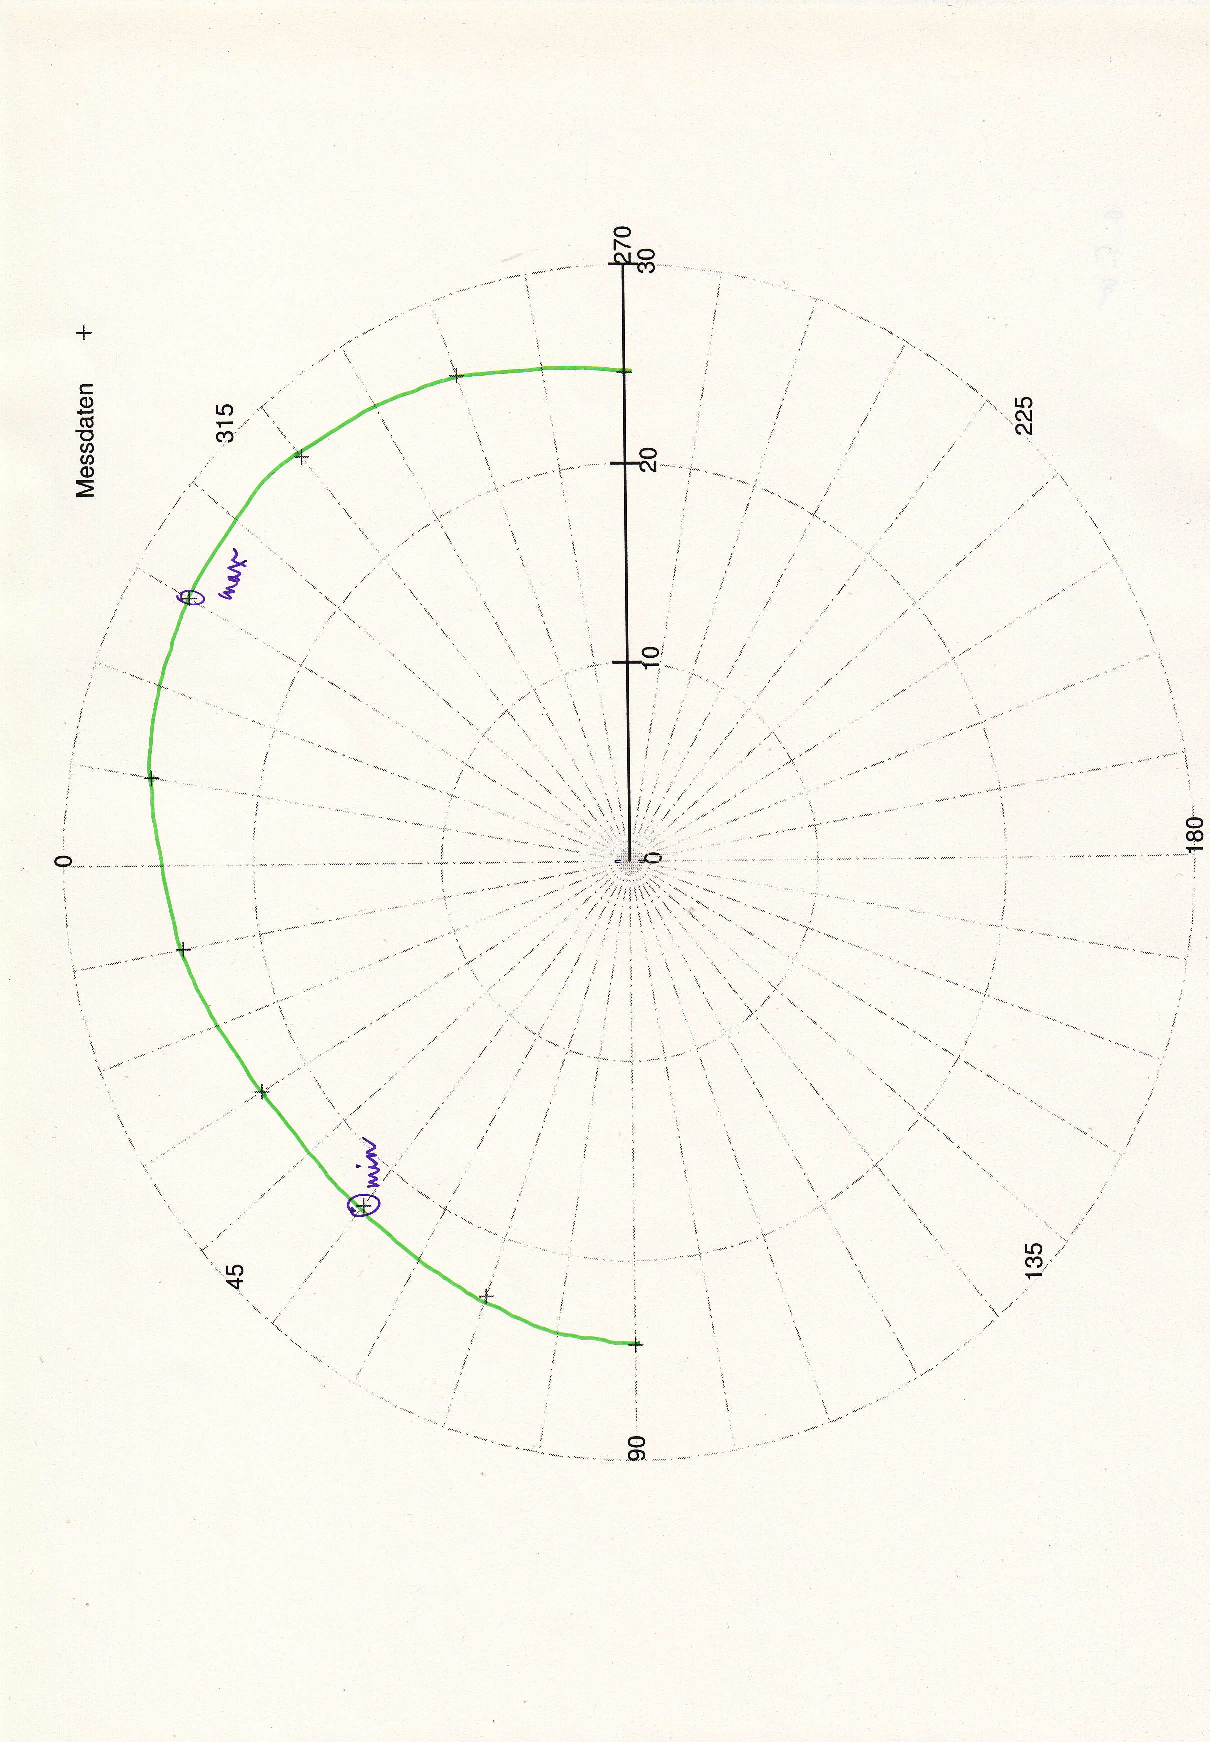
\includegraphics[scale = 0.3, angle = -90]{a_5_w.pdf}
  	\caption[Plot der Intensität in Abhängigkeit des Winkels in Polarkoordinaten, bei weißem Licht]{Plot der Intensität in Abhängigkeit des Winkels in Polarkoordinaten, bei weißem Licht}
  \label{fig:a_5_w}
\end{figure}

Es ergab sich nach Gleichung \ref{eqn:a_5_b} für den Phasenwinkel und Gleichung \ref{eqn:a_5_b_sigma} für den Fehler ein Wert von 1,569 $(\pm 0,003)$Grad.\\

Für dunkelrotes Licht ergab sich der folgend Plot (Werte aus Tabelle \ref{fig:a_5_dr}).

\begin{figure}[H]
\centering
    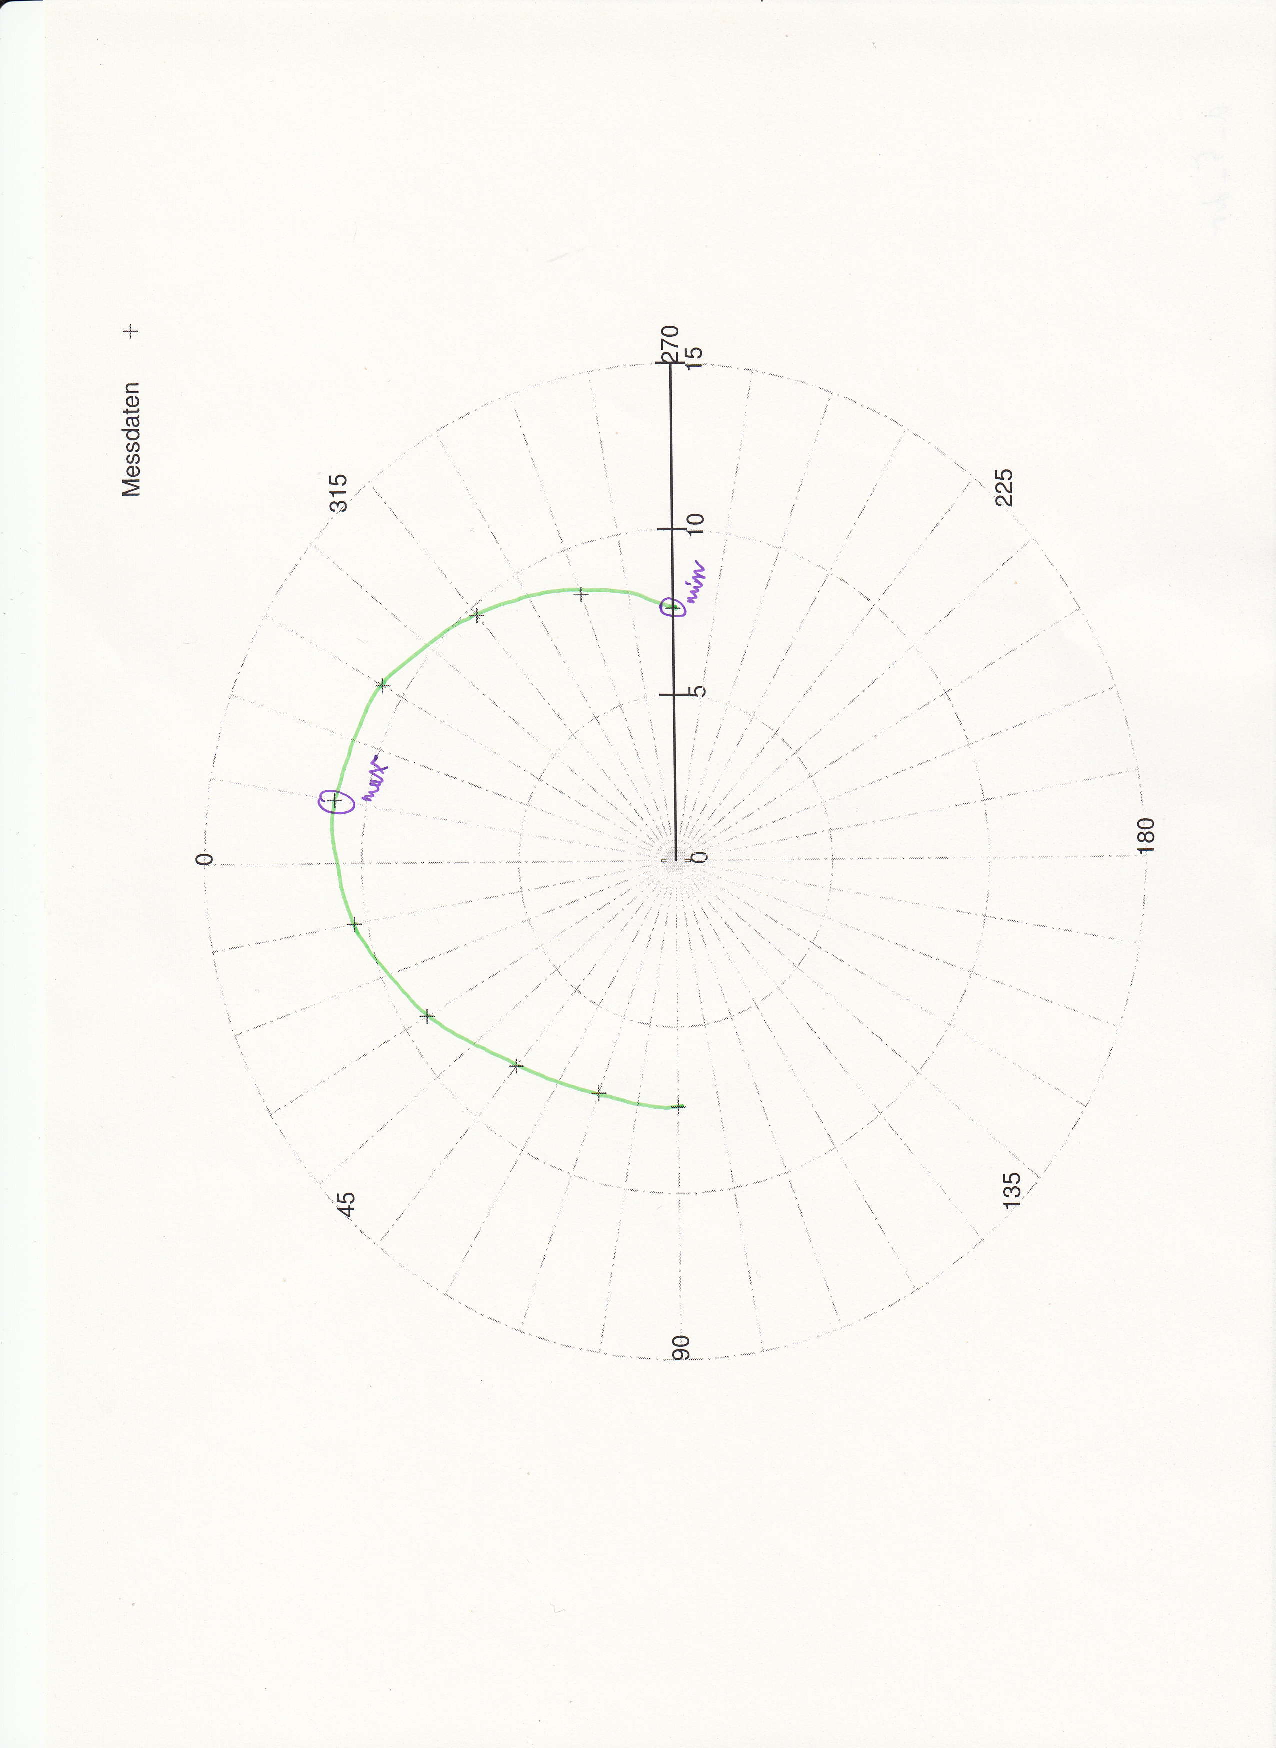
\includegraphics[scale = 0.3, angle = -90]{a_5_dr.pdf}
  	\caption[Plot der Intensität in Abhängigkeit des Winkels in Polarkoordinaten, bei dunkelrotem Licht]{Plot der Intensität in Abhängigkeit des Winkels in Polarkoordinaten, bei dunkelrotem Licht}
  \label{fig:a_5_dr}
\end{figure}

Es ergab sich nach Gleichung \ref{eqn:a_5_b} für den Phasenwinkel und Gleichung \ref{eqn:a_5_b_sigma} für den Fehler ein Wert vonn 1,567 $(\pm 0,009)$Grad.\\

Für gelbes Licht ergab sich der folgen Plot (Werte aus Tabelle \ref{tab:a_5_b_g}).

\begin{figure}[H]
\centering
    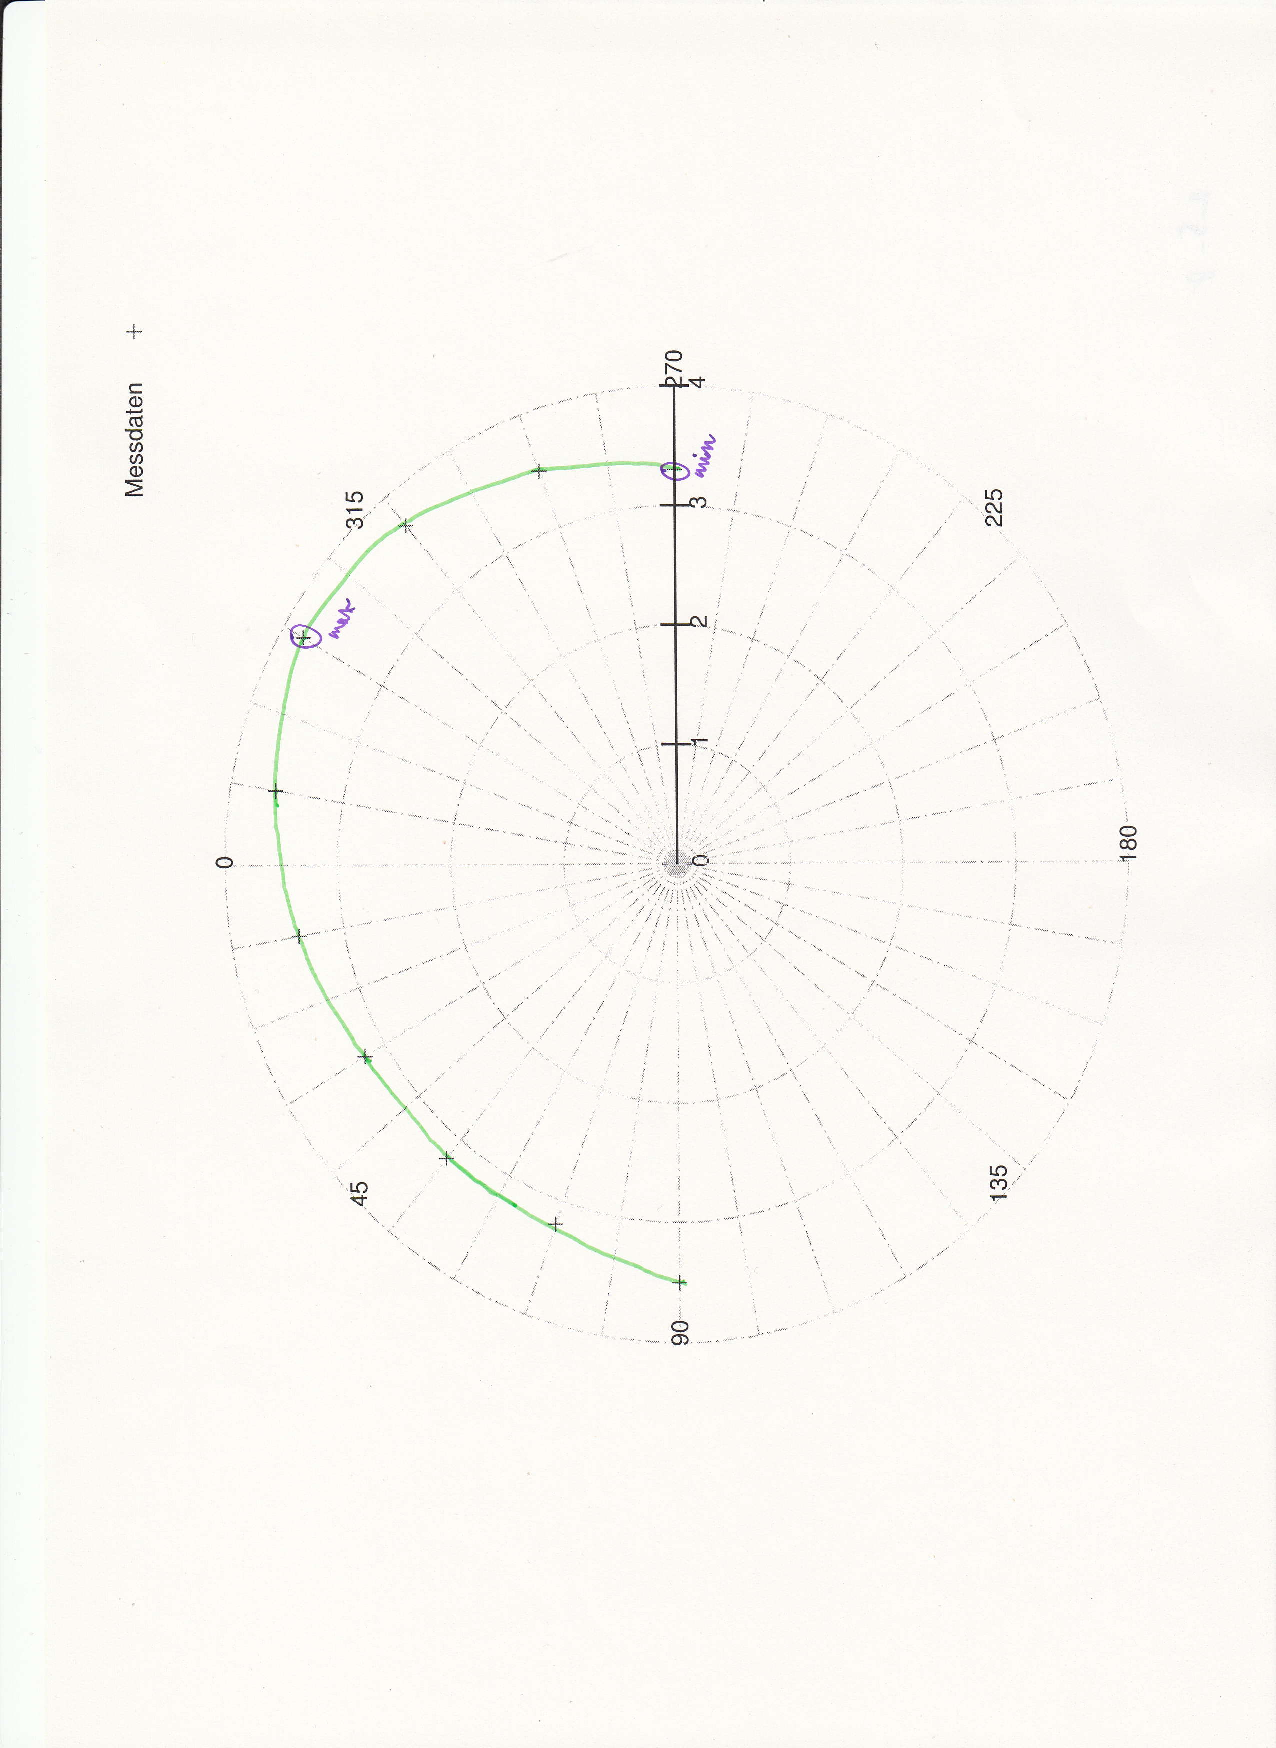
\includegraphics[scale = 0.3, angle = -90]{a_5_g.pdf}
  	\caption[Plot der Intensität in Abhängigkeit des Winkels in Polarkoordinaten, bei gelbem Licht]{Plot der Intensität in Abhängigkeit des Winkels in Polarkoordinaten, bei gelbem Licht}
  \label{fig:a_5_g}
\end{figure}


Es ergab sich nach Gleichung \ref{eqn:a_5_b} für den Phasenwinkel und Gleichung \ref{eqn:a_5_b_sigma} für den Fehler ein Wert von 1,57 $(\pm 0,02)$Grad.\\


Für gelbgrünes Licht ergab sich der folgende Plot (Werte aus Tabelle \ref{tab:a_5_b_gg}).

\begin{figure}[H]
\centering
    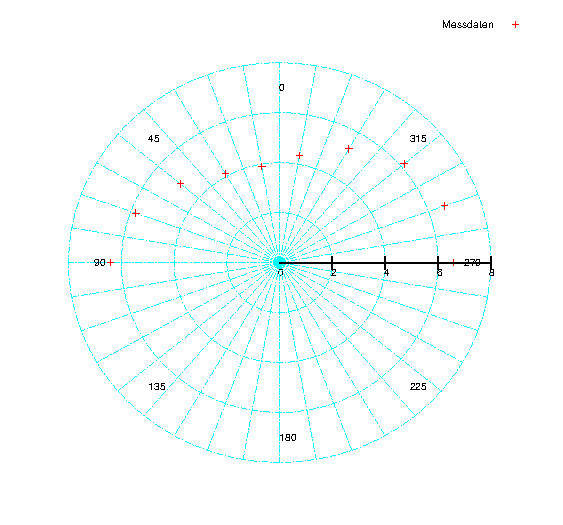
\includegraphics[scale = 0.3, angle = -90]{a_5_gg.pdf}
  	\caption[Plot der Intensität in Abhängigkeit des Winkels in Polarkoordinaten, bei gelbgrün Licht]{Plot der Intensität in Abhängigkeit des Winkels in Polarkoordinaten, bei gelbgrün Licht}
  \label{fig:a_5_gg}
\end{figure}

Es ergab sich nach Gleichung \ref{eqn:a_5_b} für den Phasenwinkel und Gleichung \ref{eqn:a_5_b_sigma} für den Fehler ein Wert von 1,57 $(\pm 0,01)$Grad.\\

Für blaugrünes Licht ergab sich der folgende Plot (Werte aus Tabelle \ref{tab:a_5_b_v}).

\begin{figure}[H]
\centering
    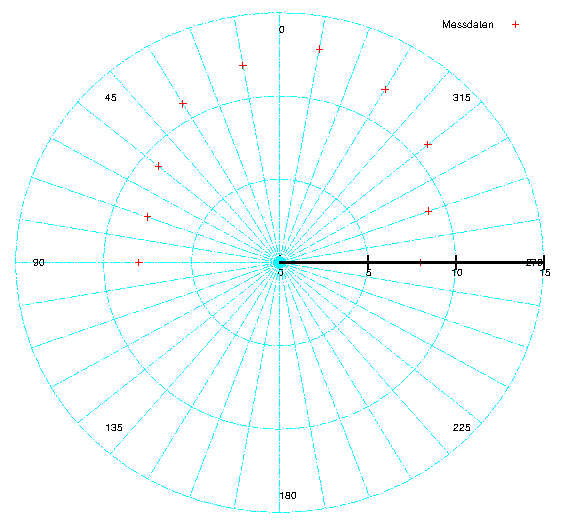
\includegraphics[scale = 0.3, angle = -90]{a_5_v.pdf}
  	\caption[Plot der Intensität in Abhängigkeit des Winkels in Polarkoordinaten, bei violettem Licht]{Plot der Intensität in Abhängigkeit des Winkels in Polarkoordinaten, bei violettem Licht}
  \label{fig:a_5_v}
\end{figure}

Es ergab sich nach Gleichung \ref{eqn:a_5_b} für den Phasenwinkel und Gleichung \ref{eqn:a_5_b_sigma} für den Fehler ein Wert von 1,568 $(\pm 0,001)$Grad.\\

Die Idealen Eingenschaften eines $\frac{\lambda}{4}$-Plättchens stellen sich bei gelbem Licht ein.

\item[c)]
Im dritten Teil der fünften Aufgabe sollte untersucht werden, was sich bei Drehung des $\frac{\lambda}{4}$-Plättchens um 90 Grad ändert. Danach sollte das Ergebnis mit der theoretischen Vorhersage verglichen werden. Für die Messung wurde der blaugrüne Filter verwendet. In den folgenden Plots wurden die Gemessenen Werte am Ursprung gespiegelt. Dabei sind die Werte oberhalb der x-Achse die "gemessenen" Werte und die unterhalb der x-Achse die "gespiegelten" Werte.(Werte aus Tabelle ??)

\begin{figure}[H]
\centering
    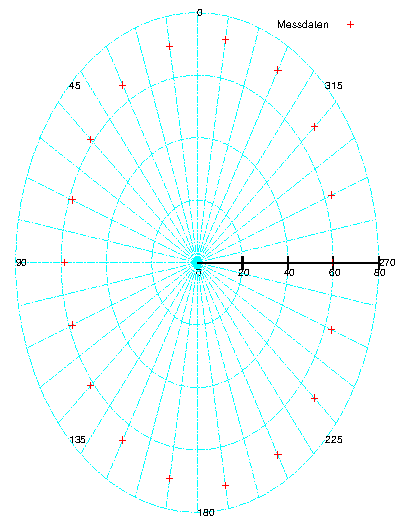
\includegraphics[scale = 1]{a_5_c.pdf}
  	\caption[Plot der Intensität in Abhängigkeit des Winkels in Polarkoordinaten, bei gelbem Licht und um 90 Grad gedrehtem $\frac{\lambda}{4}$-Plättchen]{Plot der Intensität in Abhängigkeit des Winkels in Polarkoordinaten, bei gelbem Licht und um 90 Grad gedrehtem $\frac{\lambda}{4}$-Plättchen}
  \label{fig:a_5_c}
\end{figure}


\begin{figure}[H]
\centering
    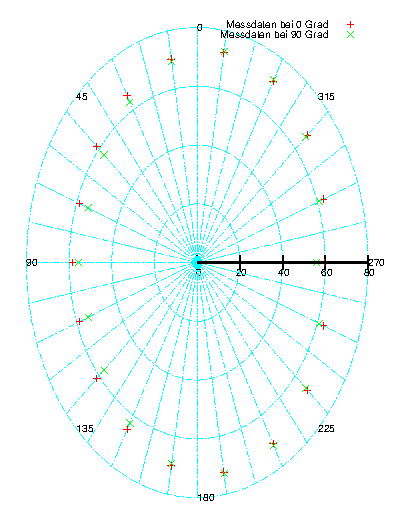
\includegraphics[scale = 1]{a_5_c_2.pdf}
  	\caption[Plot der Intensität in Abhängigkeit des Winkels in Polarkoordinaten, bei gelbem Licht und um 90 Grad gedrehtem $\frac{\lambda}{4}$-Plättchen]{Plot der Intensität in Abhängigkeit des Winkels in Polarkoordinaten, bei gelbem Licht und um 90 Grad gedrehtem $\frac{\lambda}{4}$-Plättchen}
  \label{fig:a_5_c_2}
\end{figure}

Erwartet wurde, dass sich die Polarisationsrichtung dreht, aber die beiden Kurven nicht gegeneinander verschoben sind. 


\item[d)]
Im letztem Teil der fünften Aufgabe sollte Zirkular polarisiertes Licht mit $\frac{\lambda}{4}$-Plättchen hergestellt und die Intensität bei Hintereinanderschaltung zweier Plättchen in Abhängigkeit des Winkels gemessen werden. Folgender Plot ergibt sich (Werte aus Tabelle ??).

\begin{figure}[H]
\centering
    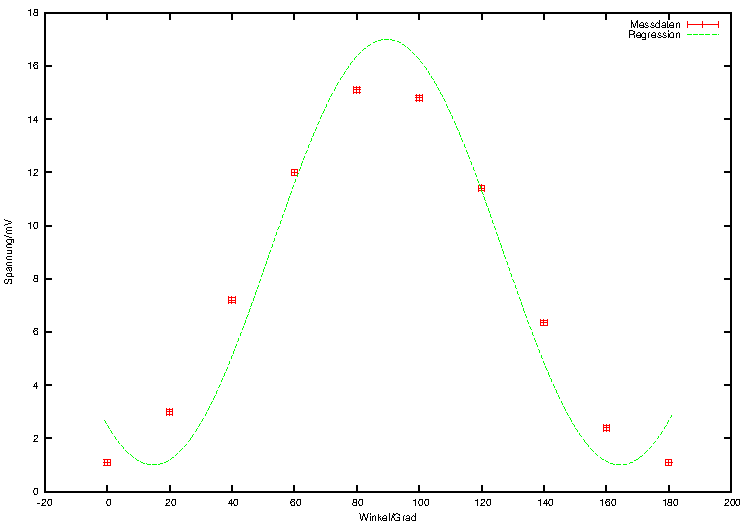
\includegraphics[scale = 1]{a_5_d.pdf}
  	\caption[Plot der Intensität in Abhängigkeit des Winkels in Polarkoordinaten, bei gelbem Licht]{Plot der Intensität in Abhängigkeit des Winkels in Polarkoordinaten, bei gelbem Licht}
  \label{fig:a_5_d}
\end{figure}
\end{enumerate}
\subsection{Diskussion}
\begin{enumerate}
\item[a)] Die gemessenen optischen Achsen des Plättchens liegen 89 Grad auseinander, bei einem Fehler von 2 Grad. Erwartet wurden 90 Grad.

\item[b)] Bei gelbem Licht haben wir festgestellt, dass das Licht näherungsweise zirkular Polarisiert war. Die berechneten Werte für die Phasenverschiebungen entsprechen nicht den Erwartungen (bei allen Messungen ein Wert von ca. 1,57 Radian), wobei nur die Beträge der Winkel ausgerechnet wurden.

\item[c)] In Aufgabenteil c) sollte das $\frac{\lambda}{4}$-Plättchen um 90 Grad verschoben und die Intensität vermessen werden. Dabei wurde erwartet, dass sich die Ellipse nicht verschiebt sondern sich nur die Drehrichtung der Welle ändert. In Abbildung \ref{fig:a_5_c_2} kann man erkennen, das die Ellipse sich bei 90 Grad Drehung des Plättchens nicht verschiebt, somit wurden die theoretischen Erwartungen durch das Experiment bestätigt.

\item[d)] Im letzten Aufgabenteil sollte zirkularpolarisiertes Licht hergestellt werden und die Intensität in Abhängigkeit der Verdrehung des zweiten Polarisators bestimmt werden. Der Plot stellt die erwartete Verteilung dar und wird gut durch den Fit approximiert.
 
\end{enumerate}


\section{Versuch WO2.2:
Bestimmung der spezifischen Drehung einer Zuckerlösung}
\subsection{Versuchsdurchführung}

\begin{figure}[H]
\centering
    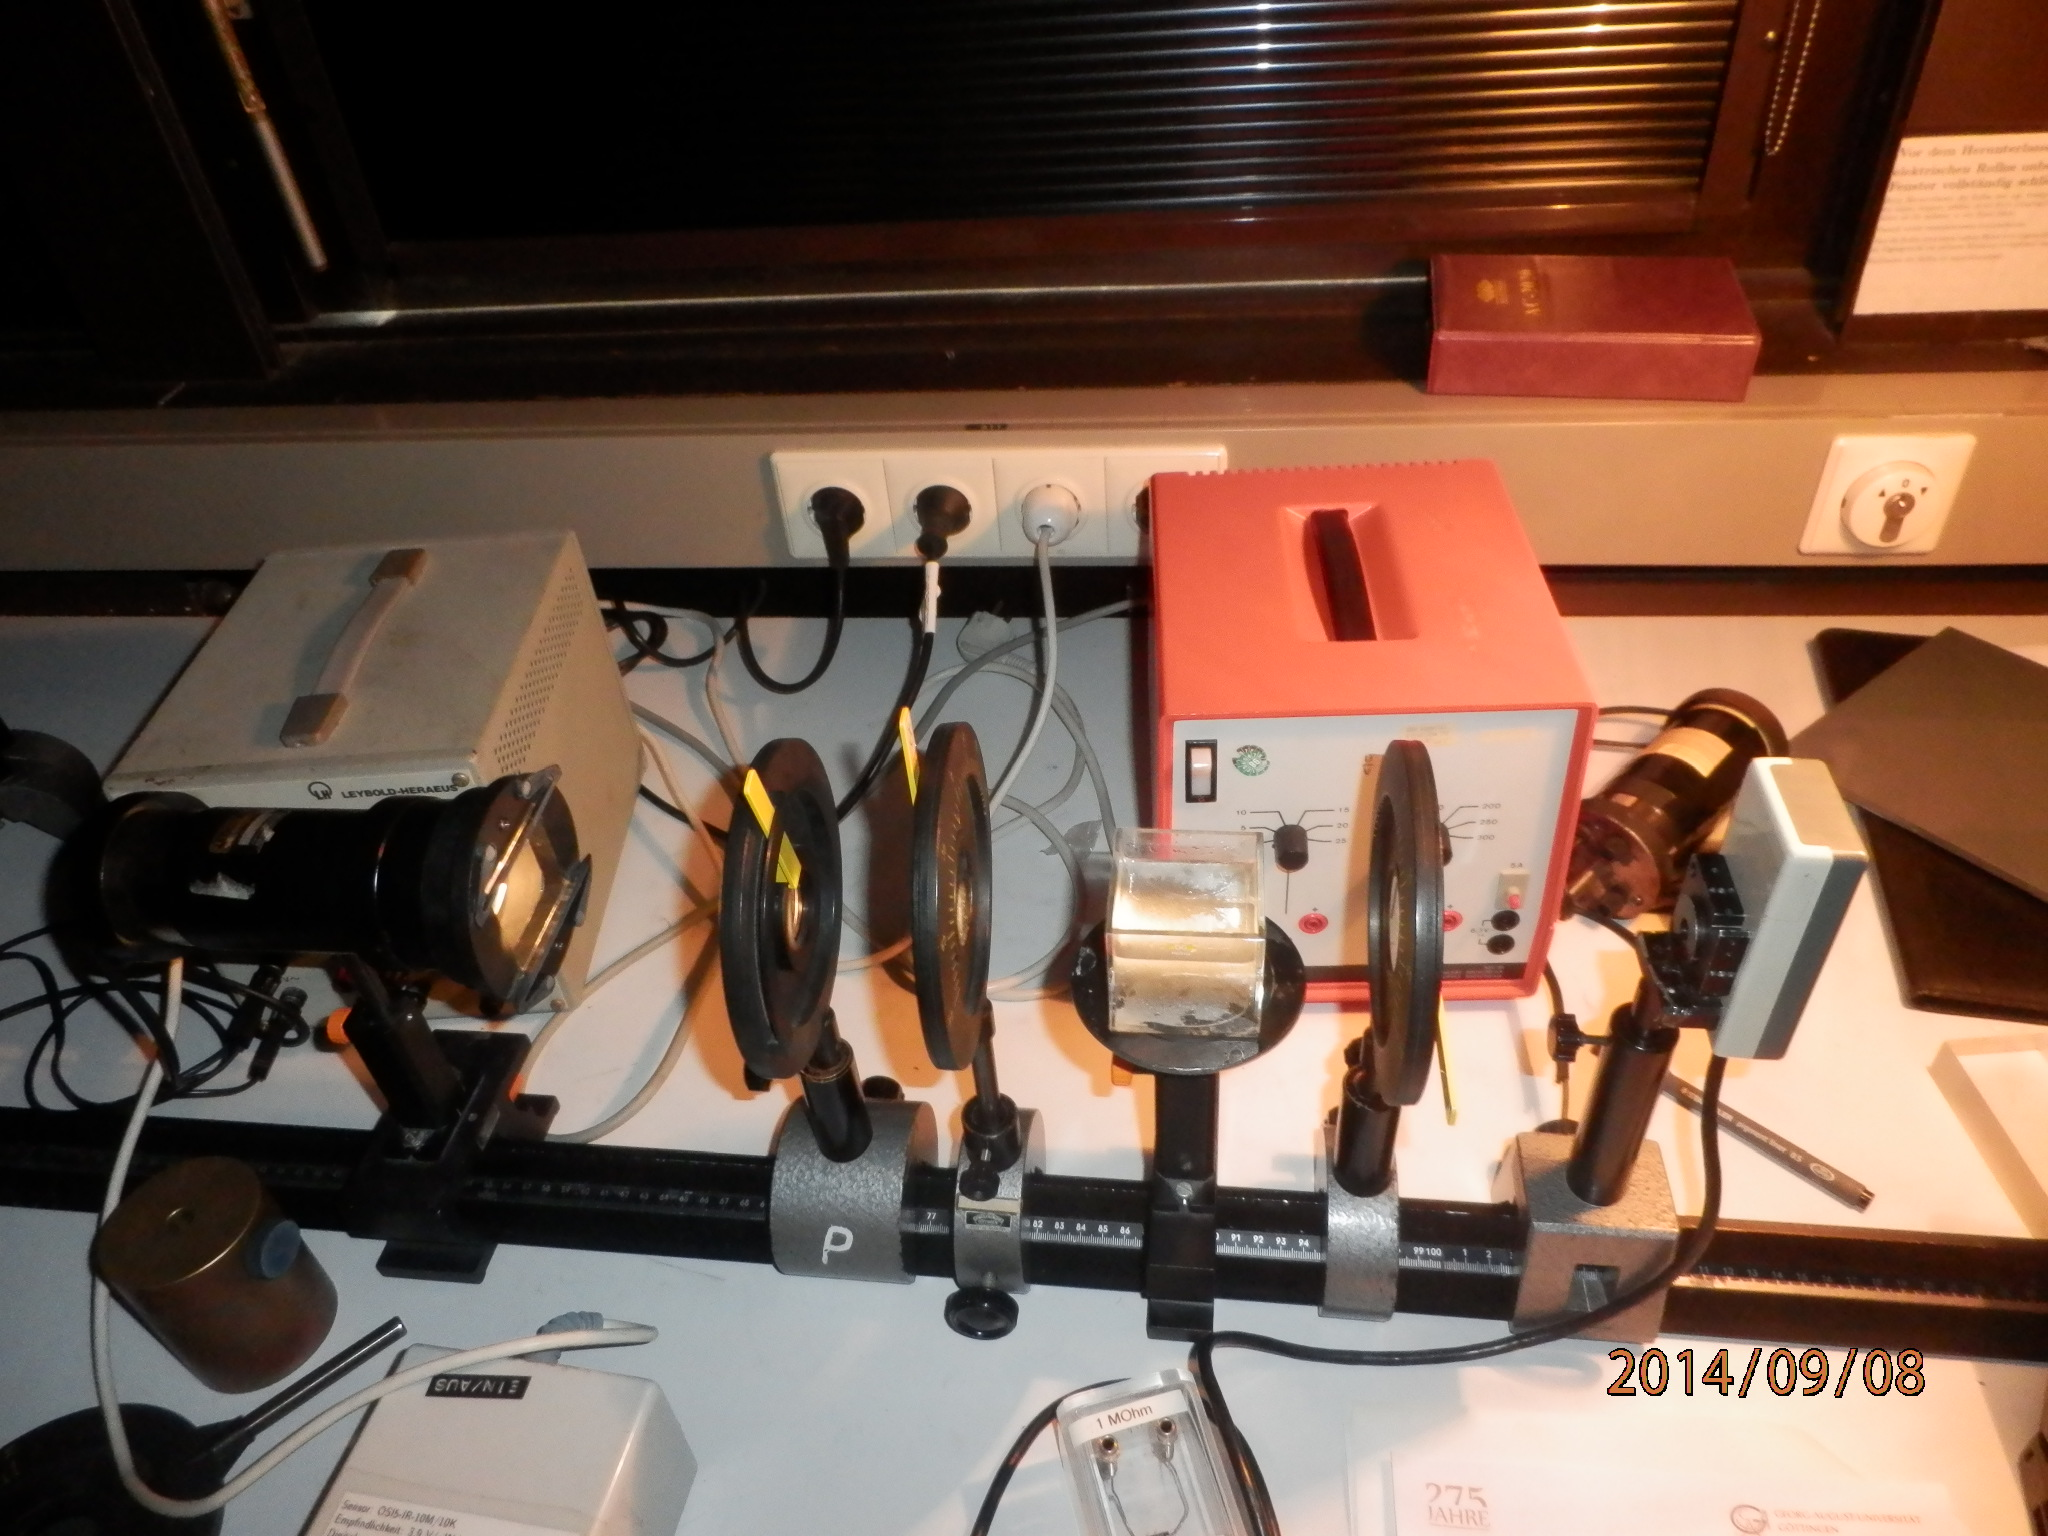
\includegraphics[scale = 0.1]{aufgabe_6.JPG}
  	\caption[Foto des Versuchsaufbaus der sechsten Aufgabe]{Foto des Versuchsaufbaus der sechsten Aufgabe}
  \label{fig:aufgabe_2}
\end{figure}

\subsubsection{Praktische Durchführung}
\begin{enumerate}
\item[a)] Wir stellen eine Zuckerlösung bekannter Konzentration q (in [$\frac{\text{g}}{\text{cm}^3}]$)
her (bis zu etwa q = 0,5$\frac{\text{g}}{\text{cm}^3}$
sind je nach Zuckersorte und Temperatur möglich).
Diese Lösung wird in einer Glasküvette zwischen zwei Polaroidfilter gestellt und die spezifische Drehung [$\alpha$]
als Funktion der Wellenlänge des Lichts bestimmt.
\item[b)] Anschließend stellen wir eine weitere Zuckerlösung mit einer anderen Konzentration als
in a) her. Mithilfe der in a) gemessenen Werte für
[$\alpha$] bestimmen wir die Konzentration dieser zweiten Zuckerlösung und vergleichen Sie mit der aus Zucker- und
Wassergewicht errechneten.
\end{enumerate}
\subsubsection{Theoretische Durchführung}
\begin{enumerate}
\item[a)] Für die spezifische Drehung [$\alpha$] gilt die Beziehung:
\begin{align}
\alpha = [\alpha] q d
\end{align}
$\alpha$ der Winkel der Polarisation des austretenden Lichtes, q die Konzentration und d die Dicke der Zuckerlösung.
Mit dem Fehler:
\begin{align}
\sigma_{[\alpha]} = \sqrt{
\left(\frac{1}{q d}\sigma_{\alpha}\right)^2+
\left(\frac{\alpha}{q^2 d}\sigma_q\right)^2+
\left(\frac{\alpha}{q d^2}\sigma_d\right)^2}
\end{align}
\item[b)]
Die Konzentration der Zuckerlösung kann aus der spezifischen Drehung [$\alpha$], der Dicke $d$ und dem Drehwinkel $\alpha$ nach folgender Formel bestimmt werden:
\begin{align}
q = \frac{\alpha}{d [\alpha]}
\label{eqn:a_6}
\end{align}
Mit dem Fehler:
\begin{align}
\sigma_q = \sqrt{
\left(\frac{1}{d [\alpha]}\sigma_\alpha \right)^2+
\left(\frac{\alpha}{d^2 [\alpha]}\sigma_d \right)^2+
\left(\frac{\alpha}{d [\alpha]^2}\sigma_{[\alpha]}\right)^2}
\label{eqn:a_6_sigma}
\end{align}
\end{enumerate}
\subsection{Messergebnisse}
\begin{table}[htbp]
\caption{Messdaten für die Bestimmung des spezifischen Winkels.}
\begin{center}
\begin{tabular}{|l|l|}
\hline
Schichtdicke/cm & Fehler/cm \\ \hline
\multicolumn{1}{|r|}{9} & \multicolumn{1}{r|}{0,1} \\ \hline
masse wasser/cm$^3$ & Fehler/m$^3$ \\ \hline
\multicolumn{1}{|r|}{65} & \multicolumn{1}{r|}{0,5} \\ \hline
masse Zucker/g & Fehler/g \\ \hline
\multicolumn{1}{|r|}{33} & \multicolumn{1}{r|}{0,5} \\ \hline
q/(g/m$^3$) & Fehler/(g/m$^3$) \\ \hline
\multicolumn{1}{|r|}{0,5076923077} & \multicolumn{1}{r|}{0,0086268861} \\ \hline
weiß &  \\ \hline
min ohne Lösung /Grad & Fehler/Grad \\ \hline
\multicolumn{1}{|r|}{90} & \multicolumn{1}{r|}{2} \\ \hline
min mit Lösung/Grad & Fehler/Grad \\ \hline
\multicolumn{1}{|r|}{7,5} & \multicolumn{1}{r|}{2} \\ \hline
blaugrün &  \\ \hline
min mit Lösung/Grad & Fehler/Grad \\ \hline
\multicolumn{1}{|r|}{7,5} & \multicolumn{1}{r|}{2} \\ \hline
rot &  \\ \hline
min mit Lösung/Grad & Fehler/Grad \\ \hline
\multicolumn{1}{|r|}{7} & \multicolumn{1}{r|}{2} \\ \hline
\end{tabular}
\end{center}
\label{tab:a_6}
\end{table}
\subsection{Auswertung}
\begin{enumerate}
\item[a)]
Im ersten Teil der sechsten Aufgabe sollte die spezifische Drehung einer Zuckerlösung für verschiedene Wellenlängen bestimmt werden. Zur Berechnung wurde Gleichung \ref{eqn:a_6} und für den Fehler Gleichung \ref{eqn:a_6_sigma} verwendet. Für weißes Licht ergab sich ein Wert von 0,34 $(\pm 0,01)$(cm$^2$/g), für blaugrünes Licht ergab sich ein Wert von 0,34 $(\pm 0,01)$(cm$^2$/g) und für dunkelrotes Licht ergab sich ein spezifischer Winkel von 0,36 $(\pm 0,02)$(cm$^2$/g).

\item[b)]
Diesen Versuchsteil haben wir aus Zeitgründen nicht geschafft.
\end{enumerate}

\subsection{Diskussion}
Es sollte die spezifische Drehung der Zuckerlösung bestimmt werden. In Aufgabenteil b sollte bei einer anderen bekannten Konzentration über die spezifische Drehung umgekehrt die Konzentration berechnet und mit dem bekannten Wert verglichen werden. Da die Zeit nicht reichte um die Messungen für Teil b) durchzuführen, ist ein Vergleich nicht möglich. Unser Wert für die  spezifische Drehung ist mit dem Wert der Nachbargruppe vergleichbar und der Fehler nimmt etwas mehr als 4\% unseres Messwertes ein.

\section{Versuch WO2.3:
Reflexion von linear polarisiertem Licht an einer Metalloberfläche}
\subsection{Versuchsdurchführung}

\subsubsection{Praktische Durchführung}
Wir haben in allen bisherigen Versuchen im Praktikum immer nur die Wechselwirkung
von Lichtwellen mit Isolatoren (Glas, Plexiglas, Kunststoff, Zuckerlösung etc.) betrach-
tet. Mit der Vorstellung von Atomen als schwingungsfähige elektrische Dipole und mithilfe der Maxwellschen Theorie waren wir in der Lage, die beobachteten Phänomene zu erklären. Diese Vorstellungen versagen jedoch, wenn wir elektromagnetische Wellen mit Wellenlängen kleiner als 10 $\mu$m und ihre Wechselwirkung mit Metallen, also Leitern, untersuchen wollen. Wollen wir also die Reflexion von Lichtwellen an Metalloberflächen untersuchen, so versagen unsere bislang erworbenen Kenntnisse. Ein gutes Verständnis der Theorie der Leitfähigkeit von Metallen im Rahmen der Festkörperphysik, die sich wiederum auf die Quantenphysik stützt, ist hierfür notwendig. Dies soll uns jedoch nicht hindern, einige experimentelle Beobachtungen über die Reflexion von linear polarisiertem Licht an einer Metalloberfläche (Oberflächenspiegel) zu machen. Wir benötigen für die Versuche neben Lichtquelle und Oberflächenspiegel ein
$\frac{\lambda}{4}$-Plättchen und zwei Polaroidfilter und
führen damit folgende Experimente aus:
Beobachtung 1: Licht, das parallel oder senkrecht zur Einfallsebene linear polarisiert ist, ändert bei der Reflexion an einem Metallspiegel seine Polarisation nicht.
Beobachtung 2: Licht, das in einem Winkel von 45$^\circ$ zur Einfallsebene linear polarisiert ist, wird durch die Reflexion in elliptisch polarisiertes Licht umgewandelt.
Beobachtung 3: Es gibt einen Einfallswinkel, bei dem
”unter 45$^\circ$
linear polarisiertes
Licht“ als nahezu zirkular polarisiert reflektiert wird.
Eine plausible Erklärung für diese Beobachtungen finden Sie im Berkeley Kurs Band 3, Kap. 8.6, Heimversuch 26.
\subsection{Auswertung}
Diesen Versuchsteil haben wir aus Zeitgründen nicht geschafft.


\section{Fazit}
Insgesamt lässt sich zu diesem Versuch sagen, dass wir bei der Auswertung als auch bei der Durchführung Zeitprobleme hatten, sodass nicht alle Zusammenhänge vollständig erklärt werden konnten. Die Aufgabenstellung in Aufgabe 5 d)
war nicht eindeutig, wodurch wir eine eigene Interpretation der Aufgabe umgesetzen mussten.
Dabei haben wir den gleichen Aufbau wie unsere Nachbargruppe analysiert.
Die Theorie aus dem Anhang der Versuchsanleitung haben wir stattdessen in Aufgabenteil b) verwendet.(was nicht sehr erfolgreich war)
Schließlich konnten trotzdem einige interessante Beobachtungen gemacht werden, wobei für präzisere Ergebnisse zu wenig Zeit zur Verfügung war.
 %Werte stimmen mit den Formeln überein/nicht überein

\end{document}

